\documentclass[12pt,a4paper]{article}
\usepackage{caption}  
\usepackage{float}
\usepackage{sectsty}
\usepackage{listings}
\usepackage{color}
\usepackage[hidelinks]{hyperref}
\usepackage{fullpage}
\usepackage{amsfonts}

\usepackage{float}
\usepackage{bookmark}
\setcounter{secnumdepth}{0}
\definecolor{dkgreen}{rgb}{0,0.6,0}
\definecolor{gray}{rgb}{0.5,0.5,0.5}
\definecolor{mauve}{rgb}{0.58,0,0.82}

\lstset{frame=tb,
  language=Java,
  aboveskip=3mm,
  belowskip=3mm,
  showstringspaces=false,
  columns=flexible,
  basicstyle={\small\ttfamily},
  numbers=none,
  numberstyle=\tiny\color{gray},
  keywordstyle=\color{blue},
  commentstyle=\color{dkgreen},
  stringstyle=\color{mauve},
  breaklines=true,
  breakatwhitespace=true
  tabsize=3
}

%\titleclass{\subsubsubsection}{straight}[\subsection]

\sectionfont{\fontsize{14}{15}\selectfont}
%\usepackage[nottoc]{tocbibind}
\floatstyle{boxed}
\usepackage{graphics,graphicx}
\textheight=247mm
\textwidth=180mm
\topmargin=-7mm
\oddsidemargin=-10mm
\evensidemargin=-10mm
\parindent 10pt
\usepackage{pgf}
\usepackage{pgfpages}

\pgfpagesdeclarelayout{boxed}
{
  \edef\pgfpageoptionborder{0pt}
}
{
  \pgfpagesphysicalpageoptions
  {%
    logical pages=1,%
  }
  \pgfpageslogicalpageoptions{1}
  {
    border code=\pgfsetlinewidth{2pt}\pgfstroke,%
    border shrink=\pgfpageoptionborder,%
    resized width=.95\pgfphysicalwidth,%
    resized height=.95\pgfphysicalheight,%
    center=\pgfpoint{.5\pgfphysicalwidth}{.5\pgfphysicalheight}%
  }%
}

\pgfpagesuselayout{boxed}
\begin{document}
%\pagestyle{plain}
\pagenumbering{arabic}
 %\renewcommand\thesection{\thechapter.\arabic{section}}
 
\parskip = \baselineskip 
\begin{center}
{\underline{\LARGE{\bf
{VLSI DESIGN LAB}
}}}
\bigskip
\bigskip
\bigskip
\\
{\Large{Report Submitted in partial fullfilment of course\\ on VLSI Design Lab (EC364)}
\\
\bigskip
\bigskip
\bigskip
Under the guidance of\\
Dr.Ramesh Kini\\
Mr.Kiran Kumar Lad

\bigskip
\bigskip

\begin{figure}[!h]
\centering

\includegraphics[scale=1.0]{images-1.jpeg}
\end{figure}

\bigskip
\vspace{10pt}
Submitted by:\\
Shah Ankit Parag 11EC86 \\ Sonawane Krunal Rajendra 11EC93
\\
\vspace{118pt}
Department Of Electronics \& Communication Engineering 
    \\National Institute Of Technology Karnataka, Surathkal 
      \\Srinivasnagar 575025 Karnataka India 

\vspace{5pt}
April 2014 }
\end{center}
\clearpage
\tableofcontents

\clearpage
\centerline{\bf
%% ENTER NAME OF PI BELOW THIS LINE
{MODULE-1 REPORT : CIRCUIT SIMULATION WITH NGSPICE}}

\bigskip

\begin{center}
%LAB1
\section{Lab 1: NMOS input, output characteristics with parametric sweeps}
%\addcontentsline{toc}{Lab 1: MOSFET input, output characteristics with parametric sweeps}
{\bf{Objective:}} 
Study the input and output characteristic of NMOS transistor. Effect of length,width,VTO,VSB,lambda, and temperature on the behavior of transistor. 
\vspace{5pt}

\begin{figure}[!h]
\centering
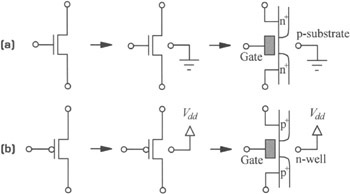
\includegraphics[scale=1.0]{nmos1.jpg}
\end{figure}
\end{center}
\textbf{Parameters:}  
\\ \textbf{Voh :} Maximum output voltage when the output level is logic "1" \\ \textbf{Vol :} Minimum output voltage when the output level is logic "0"  
\\ \textbf{Vil :} Maximum input voltage which can be interpreted as logic "0"  
\\ \textbf{Vih :} Minimum input voltage which can be interpreted as logic "1"  
\\ \textbf{Rise Time:} Time taken for output voltage to change from low to high upon change in input. 
\\ \textbf{Fall Time:} Time taken for output voltage to change from high to low upon change in input.  
\\ \textbf{Noise Margin:}  NMl = Vil - Vol  NMh = Voh - Vih
\\ \textbf{Propagation Delay:} Time it takes for the output signal voltage to switch after the input signal voltage has been applied.  
\\ \textbf{Vm:} Point on the transfer characteristics curve where Vin= Vout. 
\begin{center}
\subsection{Input Output Characteristics}
\begin{lstlisting}
m1 d g 0 0 my_nmos l = .5u w = 0.5u

*sources
v_dd d 0 dc 5
v_gg g 0 dc 3

.dc v_dd 0 5 0.1 v_gg 0 3 1
plot -v_dd#branch
end
.endc
.end

\end{lstlisting}

\begin{figure}[!ht]
\centering
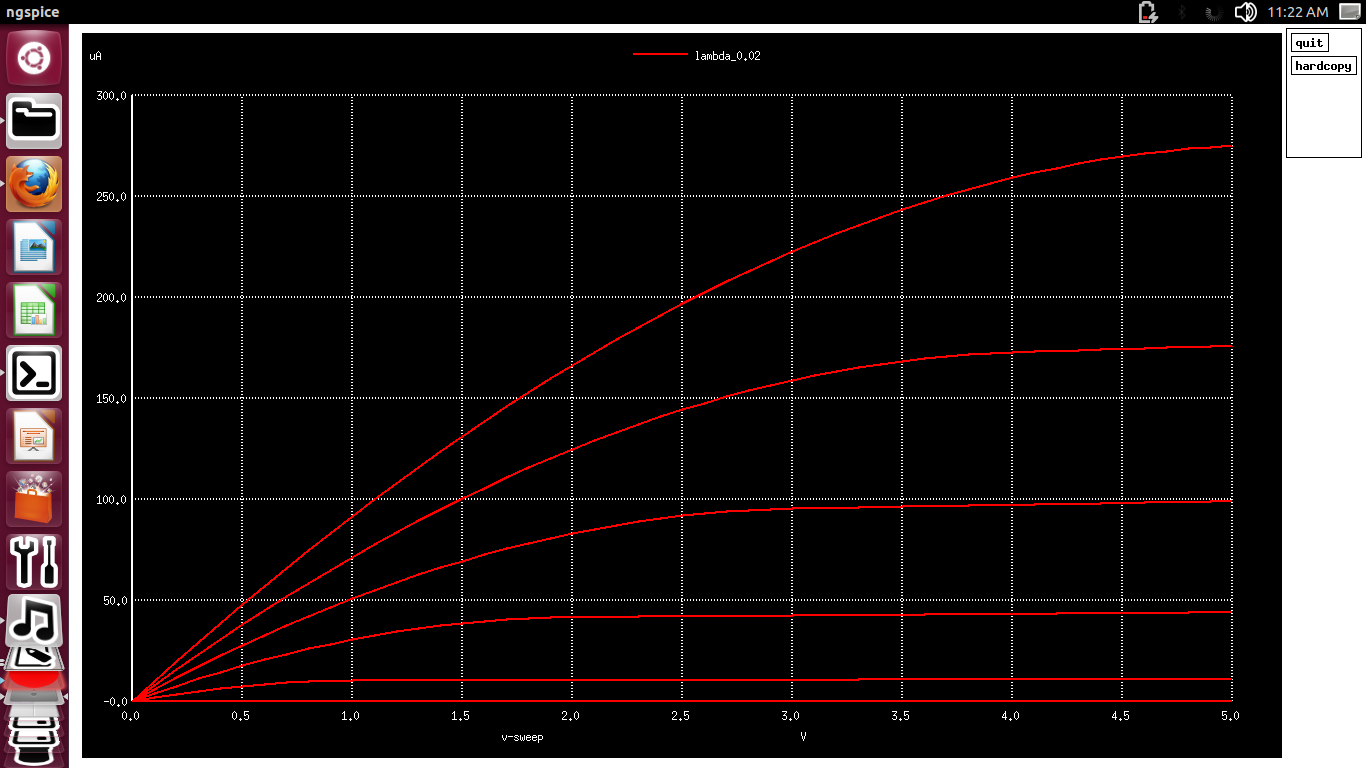
\includegraphics[scale=0.34]{lambda1a.png}
\caption[Short]{Id vs Vdd Characteristics}
\end{figure}
\vspace{15pt}
\subsection{Input Characteristics of nmos}
\begin{lstlisting}
m1 d g 0 0 my_nmos l = .5u w = 0.5u

*sources
v_dd d 0 dc 5
v_gg g 0 dc 3

.dc v_gg 0 5 0.1 
plot -v_dd#branch
end
.endc
.end

\end{lstlisting}
\clearpage
\begin{figure}[!ht]
\centering
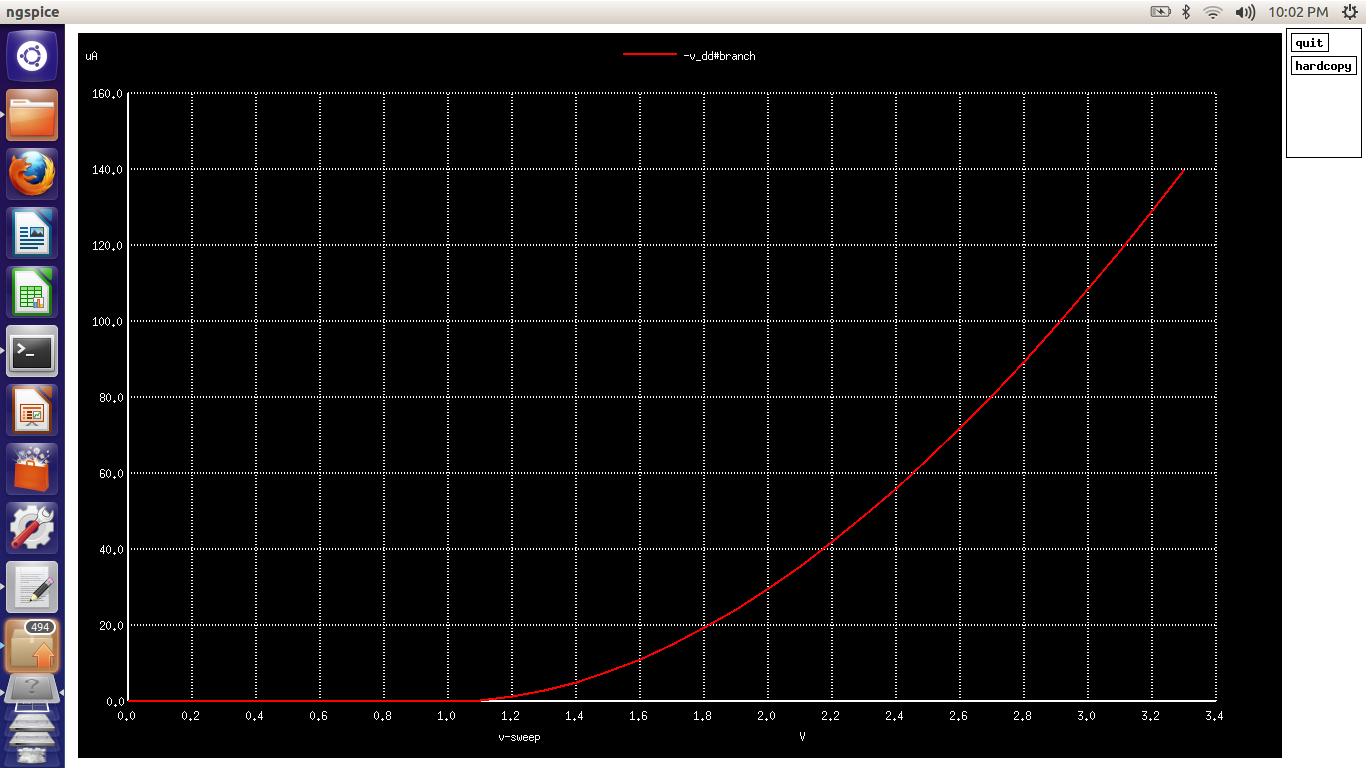
\includegraphics[scale=0.34]{lab1.png}
\caption[Short]{Input Characteristics}
\end{figure}

\subsection{Varying Lambda Id vs Vdd}
%%%%%%%%%%%%%%%%%%%%%%%%%
\begin{lstlisting}
m1 d g 0 0 my_nmos l = .5u w = 0.5u

*sources
v_dd d 0 dc 5
v_gg g 0 dc 3

.dc v_dd 0 5 0.1 v_gg 0 3 1

*response for various lambda 

.control
foreach lmda .01 .05 .09
altermod m1 LAMBDA=$lmda
run
end 
.endc
\end{lstlisting}


\begin{figure}[!ht]
\centering
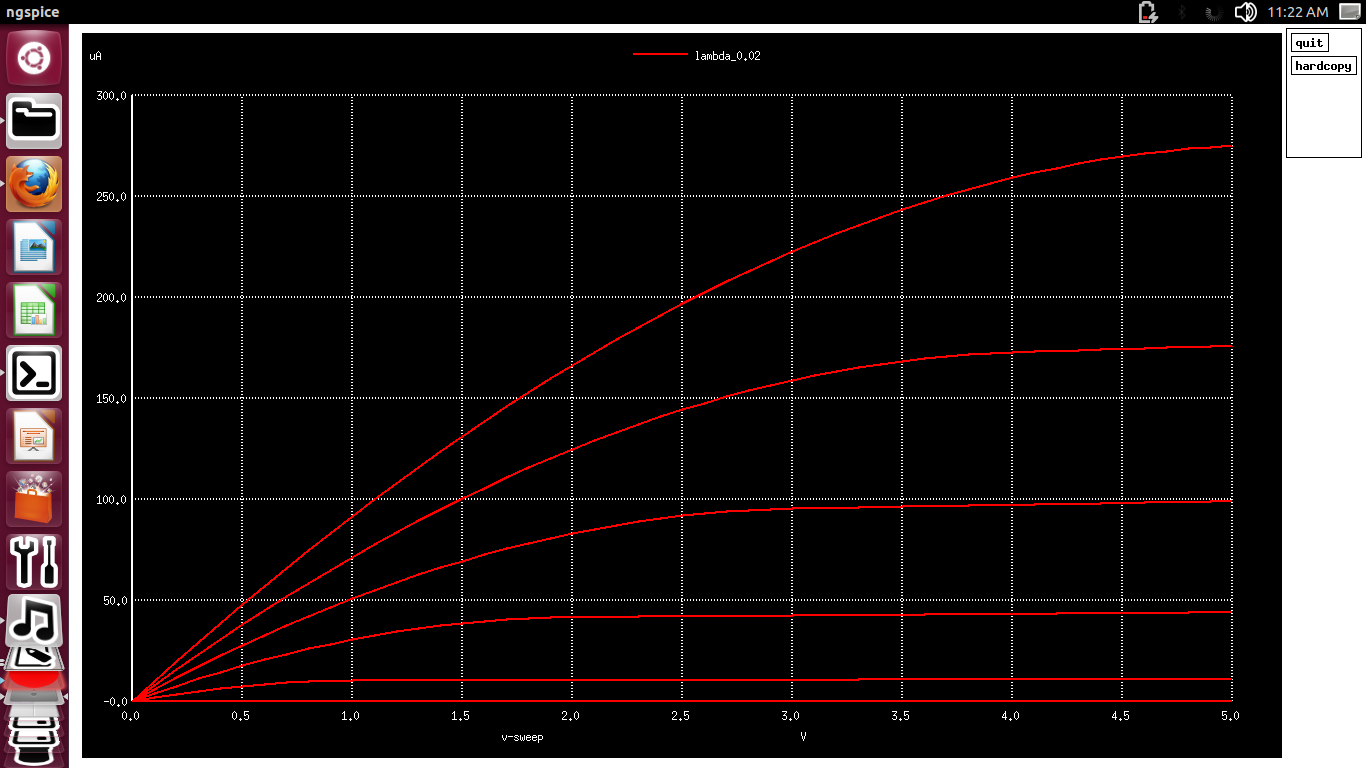
\includegraphics[scale=0.34]{lambda1a.png}
\caption[Short]{Id vs Vdd for lambda 0.01}
\end{figure}

\begin{figure}[!ht]
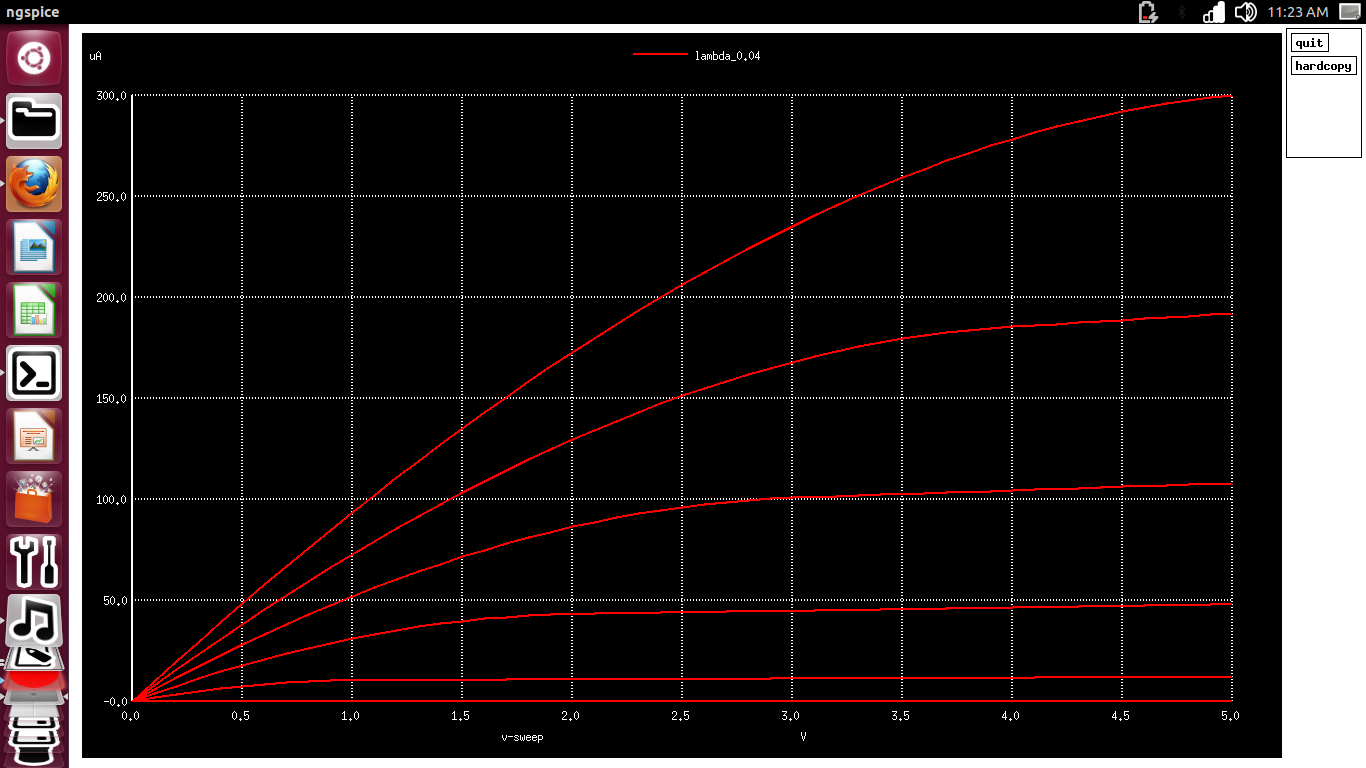
\includegraphics[scale=0.32]{lambda1b.png}

\caption[Short]{Id vs Vdd for lambda 0.05}
\end{figure}
\clearpage
\begin{figure}[h]
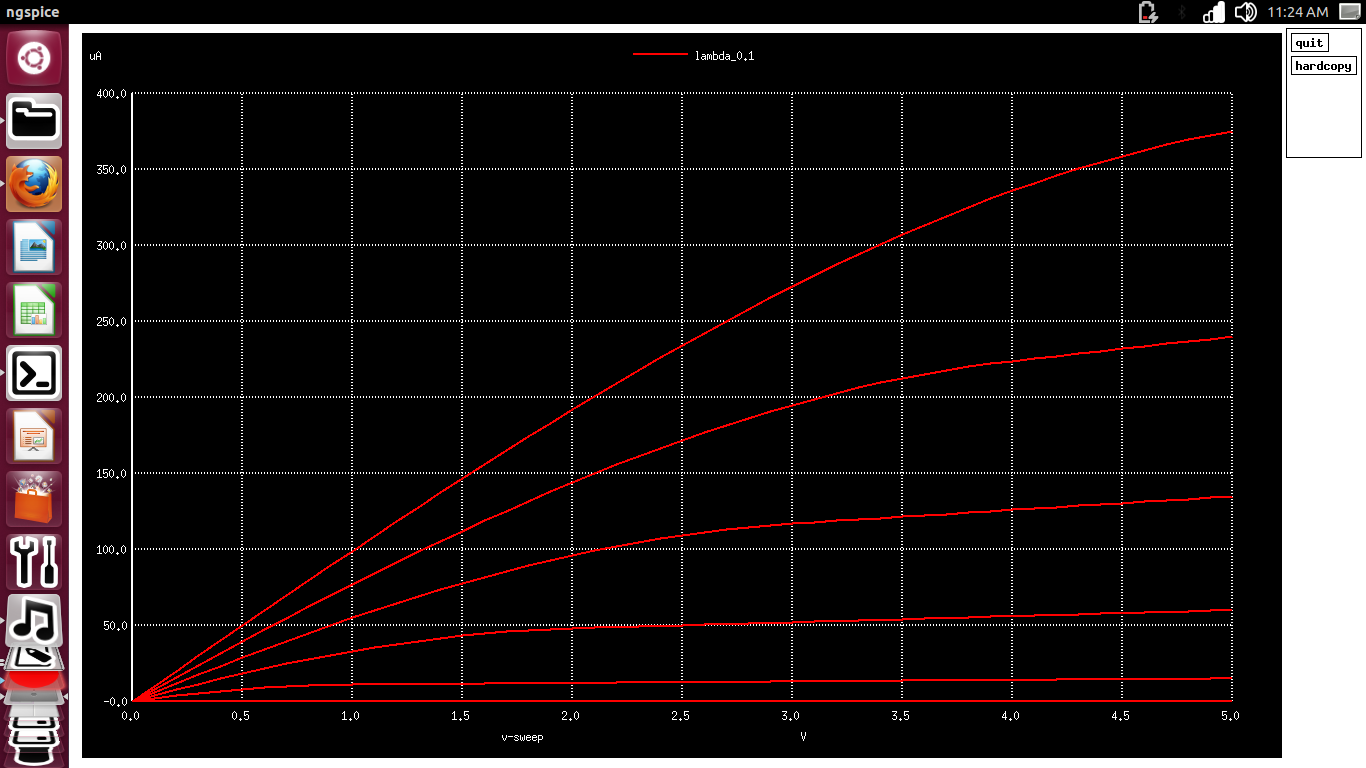
\includegraphics[scale=0.34]{lambda1c.png}
\caption[Short]{Id vs Vdd for lambda 0.09}
\end{figure}
\begin{lstlisting}
.control	
foreach iter 1 2 3
setplot dc$iter
plot -v_dd#branch
end
.endc
.end

\end{lstlisting}


\vspace{5pt}
Reason : The Id vs Vdd curve is at first linear then becomes varies slowly in saturation region 
due to channel length modulation which should be otherwise constant. 

\clearpage
\subsection{Varying Temperature}
%%%%%%%%%%%%%%%%%%%%%%%%%
\begin{lstlisting}

.include /home/Ankit/Desktop/11ec86-93/t14y_tsmc_025_level1.txt
m0 out in Vss 0 RITSUBN1 TEMP=27

*sources
Vgng Vss 0 dc 0
vdd out 0 dc 5
Vin in 0  dc  5

.dc Vin 0 5 .1
.control
foreach t1 27 50 100
alter m0 TEMP =$t1
run
end 
.endc

\end{lstlisting}

\begin{figure}[!ht]
\centering
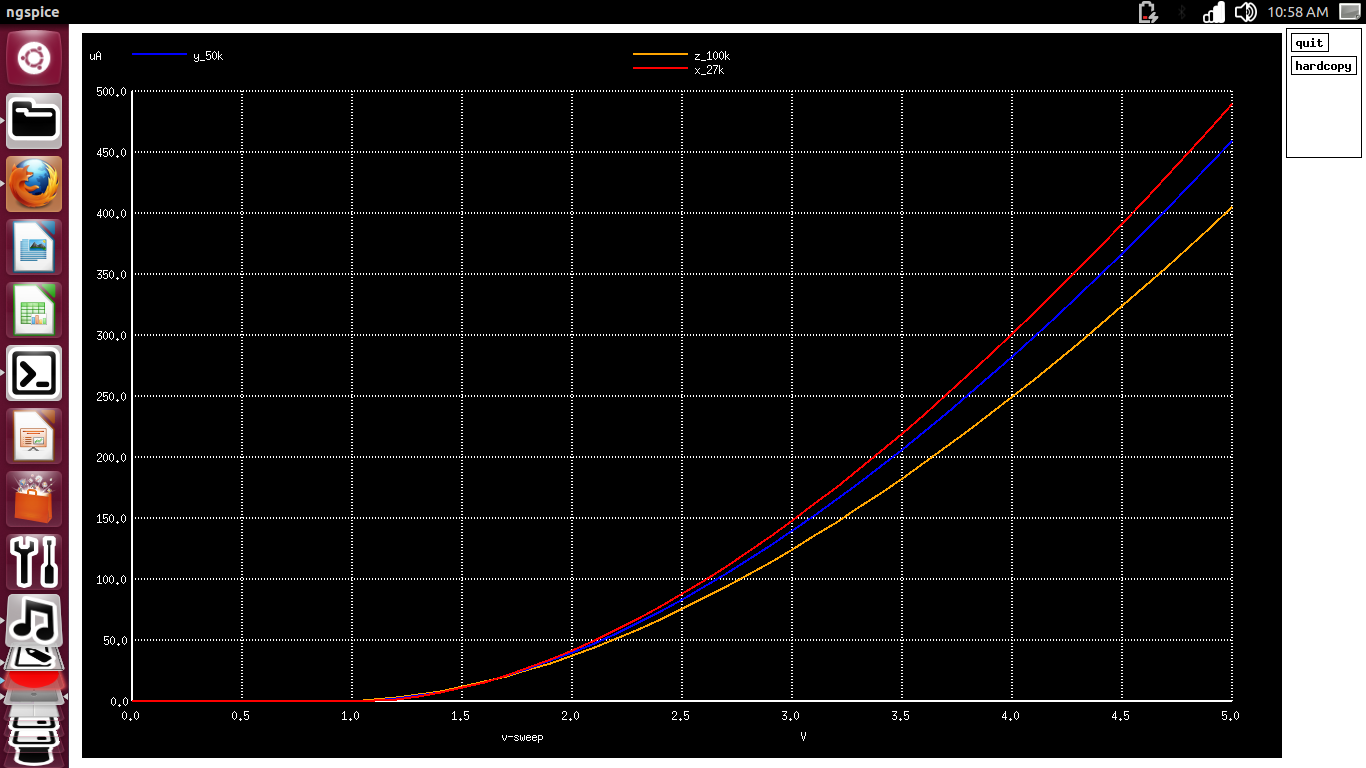
\includegraphics[scale=0.37]{temp_vary_pic.png}
\caption[Short]{Temperature Variation}
\end{figure}
\clearpage


\begin{figure}[!ht]
\centering
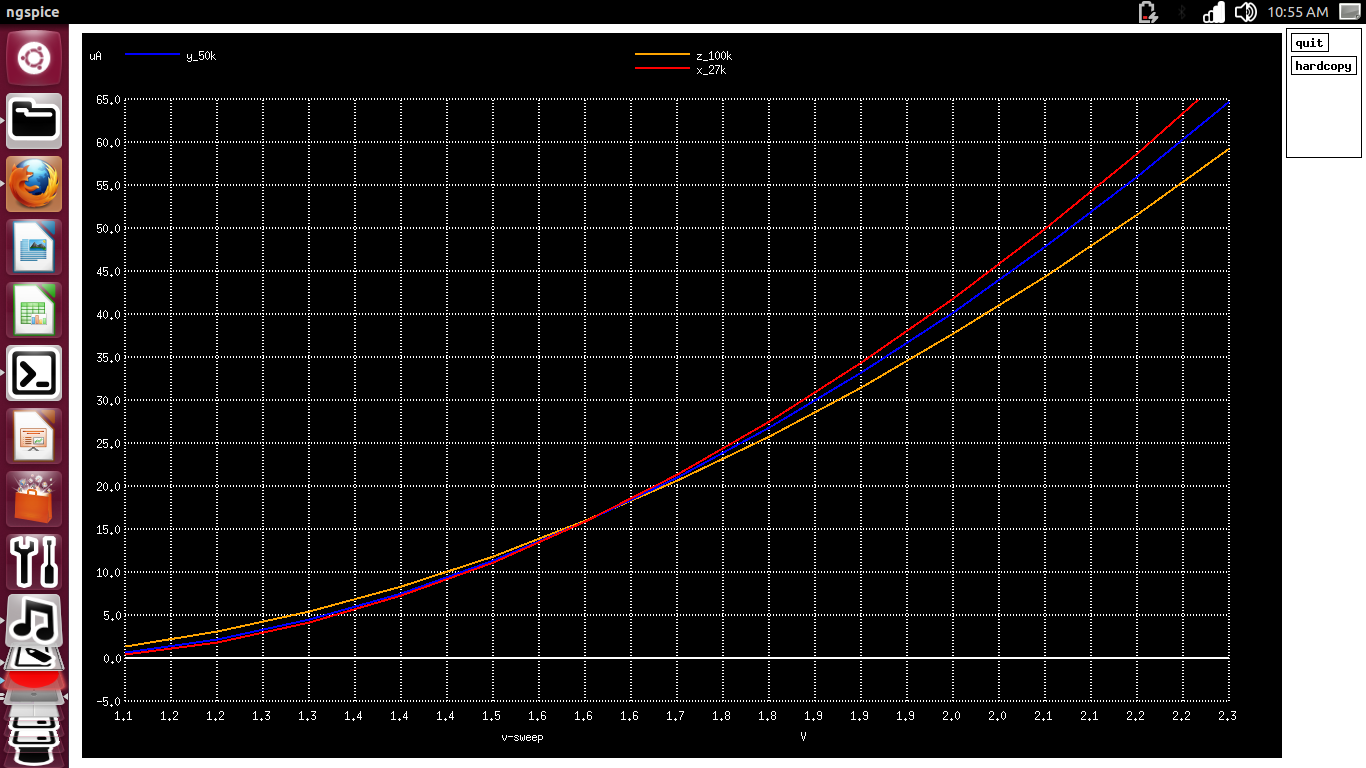
\includegraphics[scale=0.37]{temp_vary_zoomed_pic2.png}

\caption[Short]{Temperature Variation Flipover of curv (zoom)}
\end{figure}
\textit{Conclusion:} In the above figure for VI characteristics, as the value of temperature increases, the current decreases. Hence, the current is inversely proportional to the temperature.
\\
\subsection{Varying Length}
%%%%%%%%%%%%%%%%%%%%%%%%%
\begin{lstlisting}
*nmos characteristics varing length

*include model files

.include /home/krunal/VLSI_LAB/t14y_tsmc_025_level1.txt

*netlist
m1 drain gate 0 0 RITSUBN1 l=3u w=0.5u

*define the sources
vdd drain 0 dc 5
vgg gate 0 dc 5
.dc vdd 0 5 0.1 vgg 0 5 1

*Computing the response for various width('len' variable)
.control
foreach len 1.5e-6 6e-6 3e-5
alter m1 l = $len
run 
end
.endc

*plotting the output for various length
.control
foreach iter 1 2 3
setplot dc$iter
plot -vdd#branch
end
.endc


\end{lstlisting}

\begin{figure}[!ht]
\centering
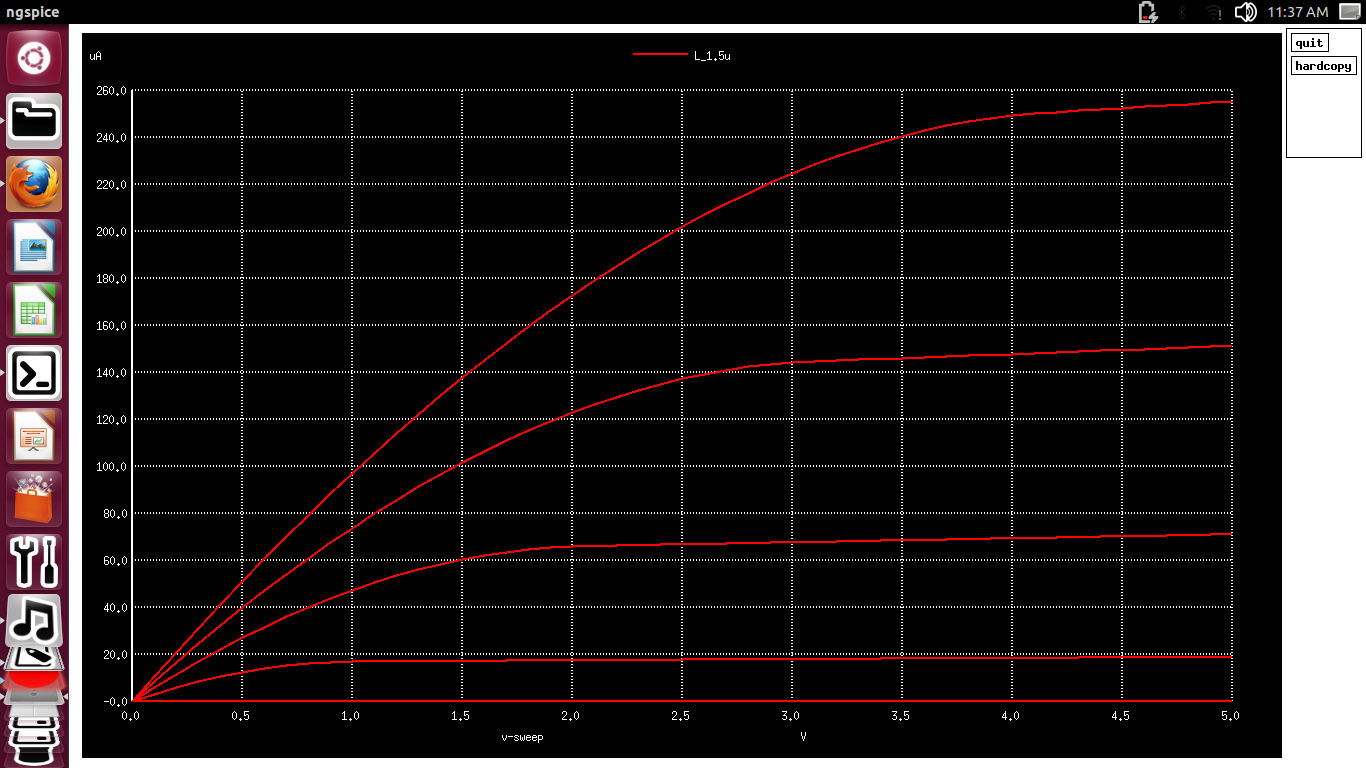
\includegraphics[scale=0.34]{vary_len_1_5.png}

\caption[Short]{For Length 1.5u}
\end{figure}

\begin{figure}[!ht]
\centering
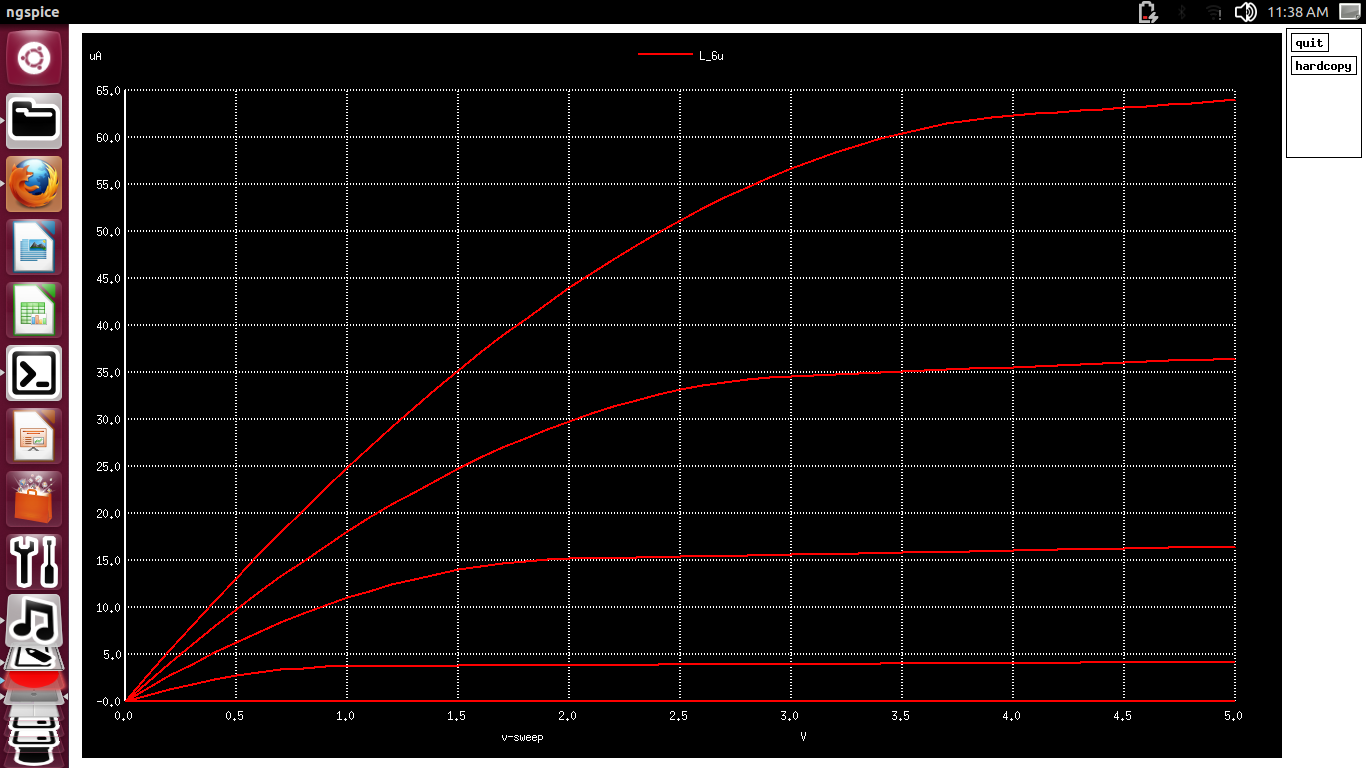
\includegraphics[scale=0.34]{vary_len_6.png}
\caption[Short]{For Length 6u}
\end{figure}

\begin{figure}[!ht]
\centering
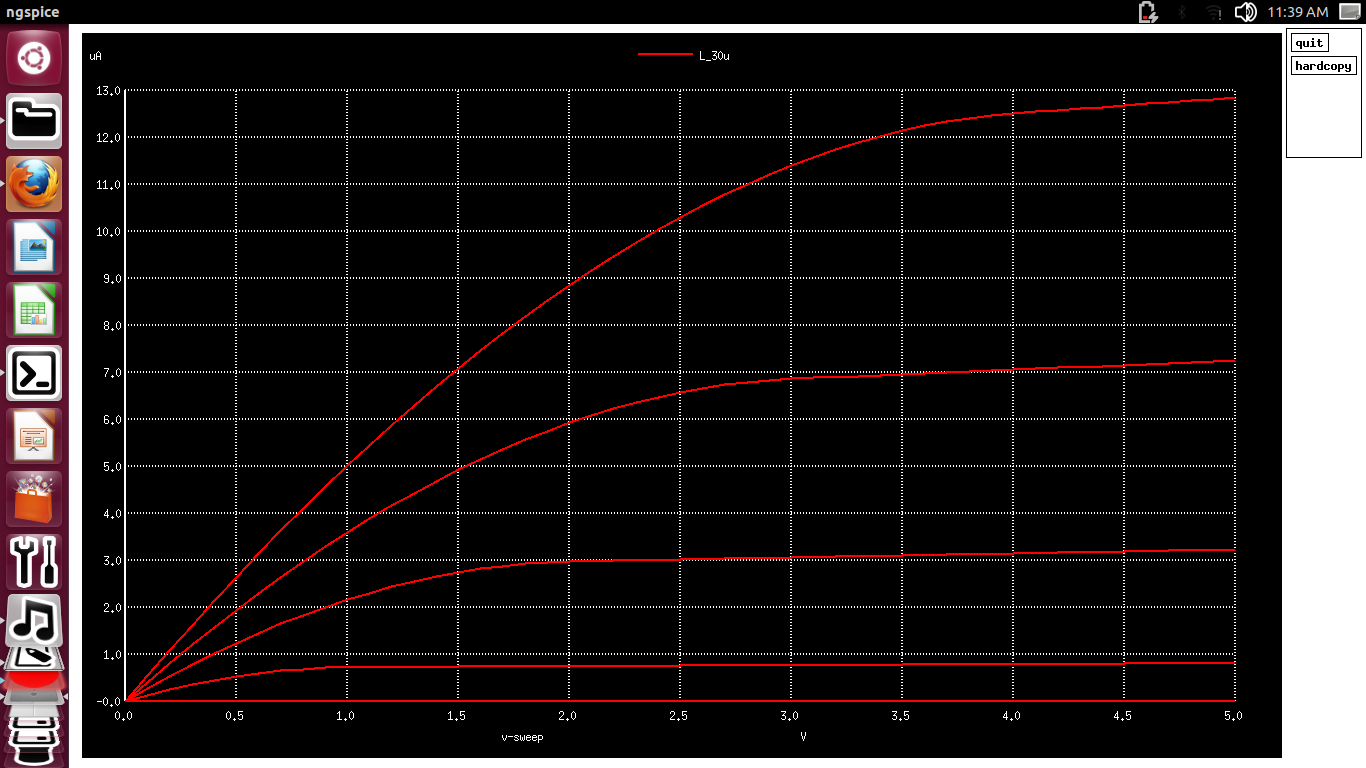
\includegraphics[scale=0.37]{vary_len_30.png}
\caption[Short]{For Length 30u}
\end{figure}

\textit{Conclusion:}  In the above figure for the VI characteristics. With increase in the value of L, the drain current decreases as shown. 
\clearpage
\subsection{Varying VTO}

%%%%%%%%%%%%%%%%%%%%%%%%%
\begin{lstlisting}

.include /home/krunal/VLSI_LAB/t14y_tsmc_025_level1.txt
.model my_nmos nmos LEVEL=1 VTO=.03
m0 out in Vss 0 my_nmos

*sources
Vgnd Vss 0 dc 0
vdd out 0 dc 5

*input_source
Vin in 0 dc 5
.dc Vin 0 5 .1

.control
foreach res 0.5 1 2
altermod m0 VTO= $res
run
end
.endc

.control
foreach iter 1 2 3
setplot dc$iter
plot -vdd#branch
end
.endc
\end{lstlisting}
\begin{figure}[!ht]
\centering
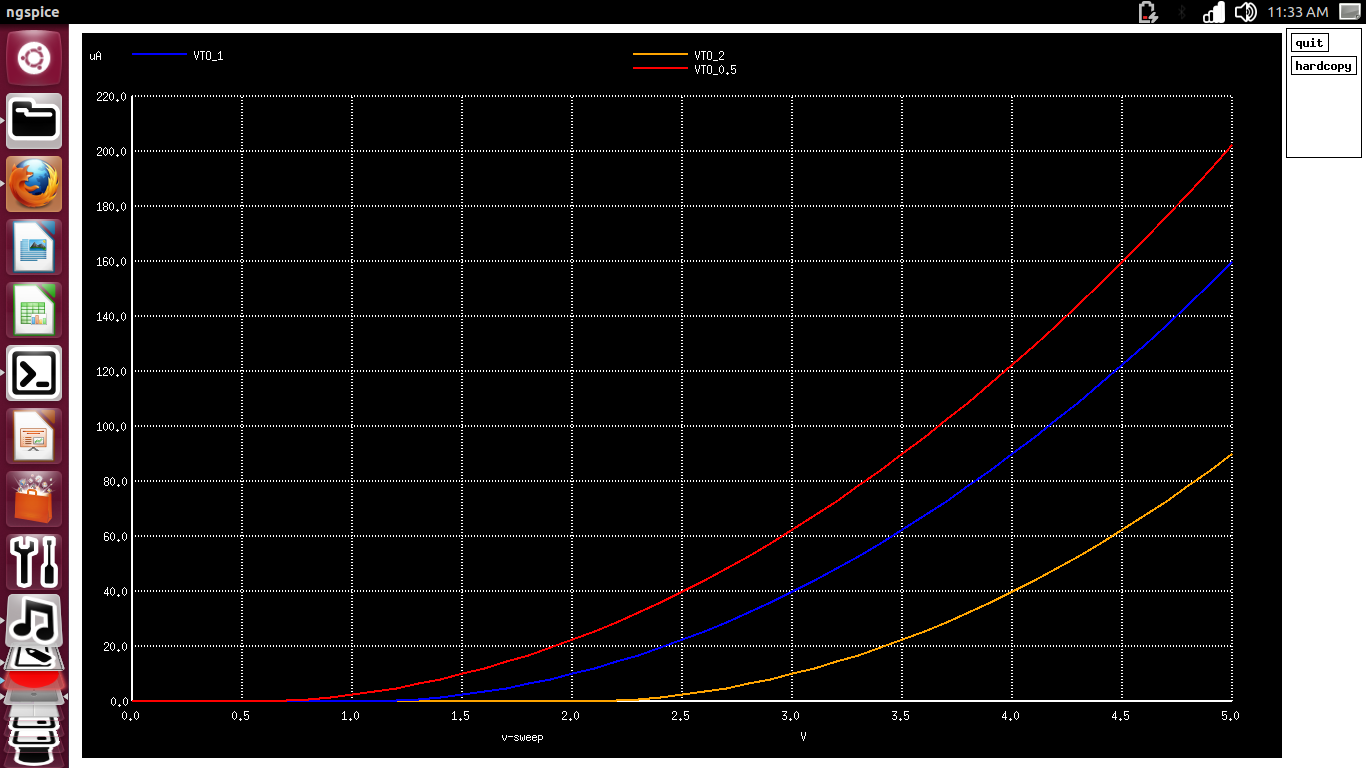
\includegraphics[scale=0.3]{vary_VTO.png}

\caption[Short]{For Varying VTO}
\end{figure}
\vspace{3pt}
\textit{Conclusion :}  In the above figure for VI characteristics, As the value of  VTo increases, the current decreases. Hence, the current is inversely proportional to VTo. \\
\vspace{3pt}
\subsection{Varying VSB}

%%%%%%%%%%%%%%%%%%%%%%%%%
\begin{lstlisting}

.include /home/krunal/VLSI_LAB/t14y_tsmc_025_level3.txt
m1 drn gate s 0 cmosn l=1u w=.5u

vdd drn 0 5
vin gate 0 5
vss s 0 0

.dc  vin 0 6 .1 vss 0 3 1
.control
run 
plot -vdd#branch
.end

\end{lstlisting}
\begin{figure}[!ht]
\centering
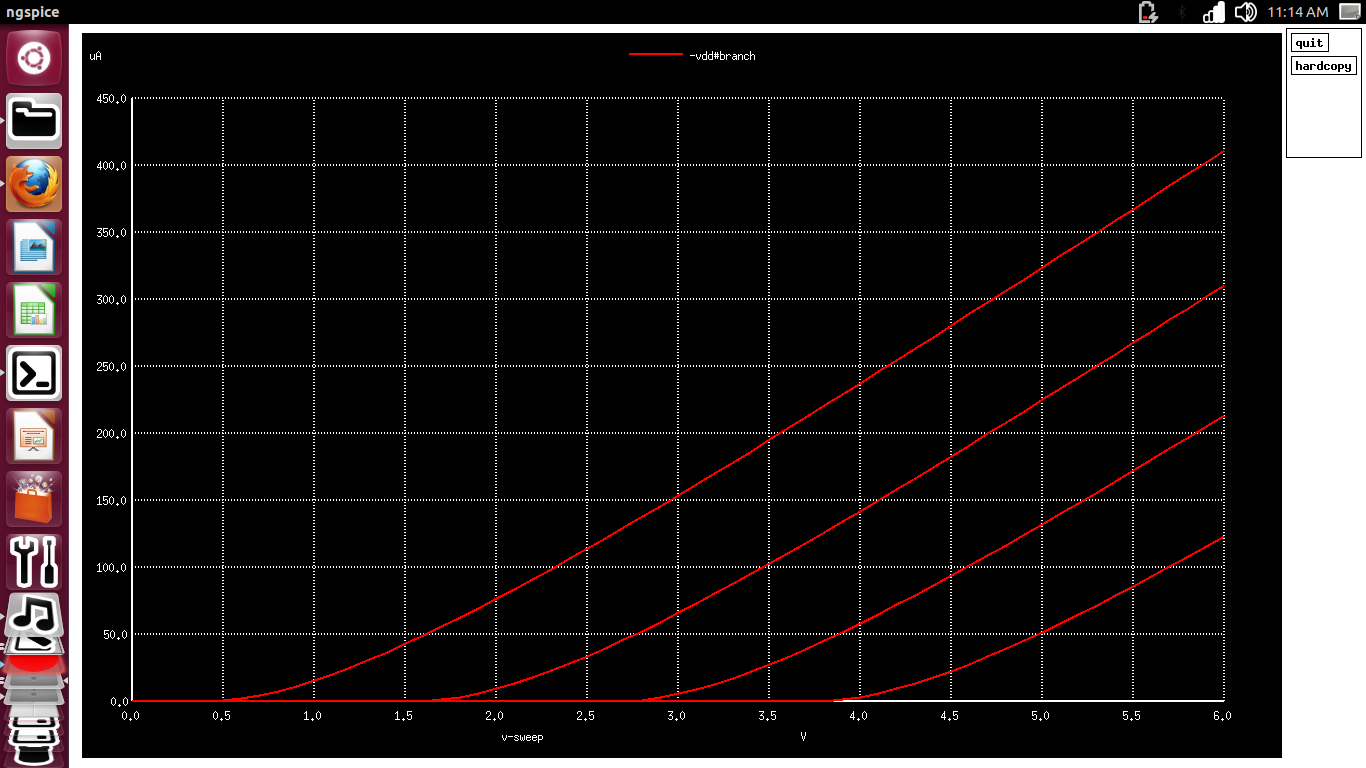
\includegraphics[scale=0.34]{VSB_vary.png}

\caption[Short]{For varying VSB}
\end{figure}

\subsection{Varying Width}

%%%%%%%%%%%%%%%%%%%%%%%%%
\begin{lstlisting}
*nmos characteristics
.include /home/krunal/VLSI_LAB/t14y_tsmc_025_level1.txt

*netlist
m1 drain gate 0 0 RITSUBN1 l=3u w=0.5u

*define the sources
vdd drain 0 dc 5
vgg gate 0 dc 5
.dc vdd 0 5 0.1 vgg 0 5 1

*Computing the response for various width
.control
foreach wid 1e-6 3e-6 5e-6
alter m1 w = $wid
run 
end
.endc

*plotting the output for various width
.control
foreach iter 1 2 3
setplot dc$iter
plot -vdd#branch
end
.endc
\end{lstlisting}

\begin{figure}[!ht]
\centering
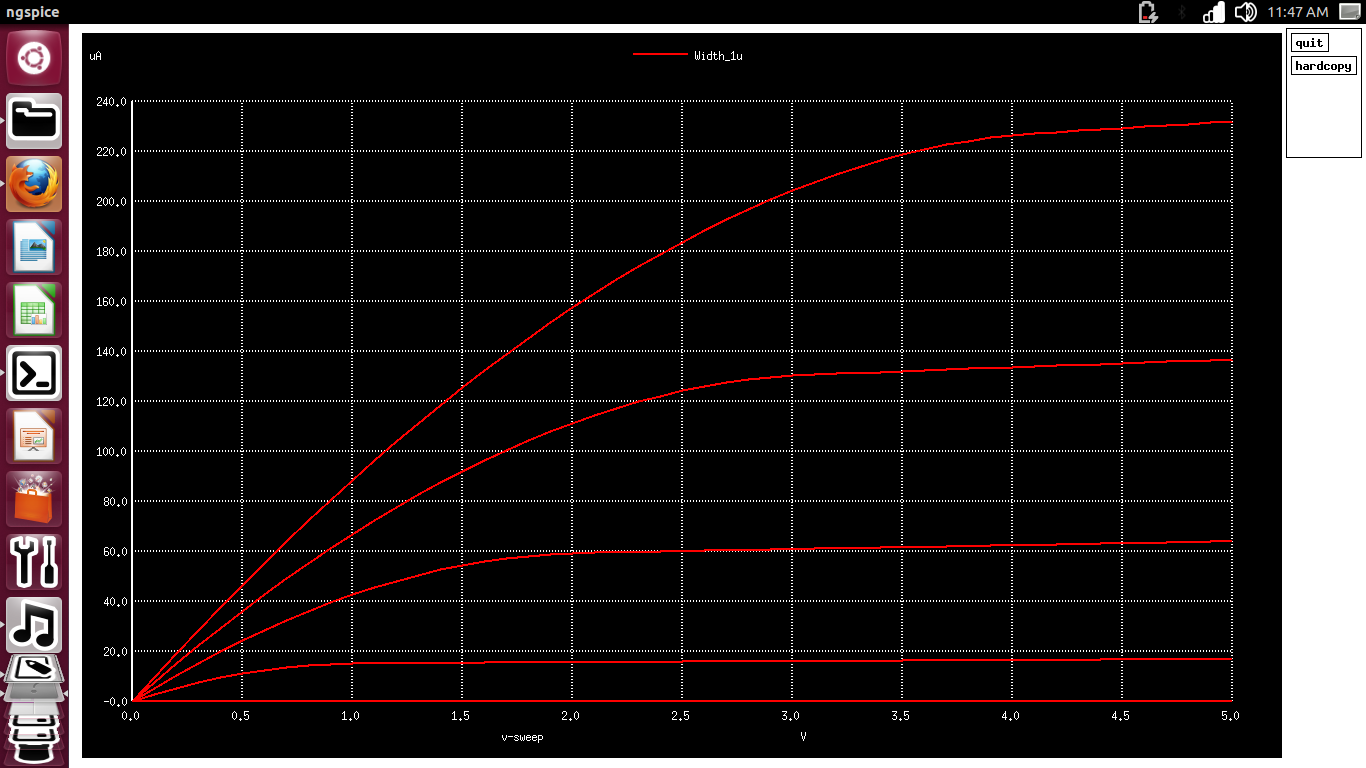
\includegraphics[scale=0.34]{width_1a.png}
\caption[Short]{For varying Width}
\end{figure}

\textit{Conclusion:}  In the above figure for the VI characteristics. With increase in the value of W, the drain current increases as shown. 
\vspace{3pt}

\begin{figure}[!ht]
\centering
\caption[Short]{For varying Width}
\includegraphics[scale=0.29]{Width_1a.png}
\caption[Short]{For  Width = 1u}
\includegraphics[scale=0.29]{Width_1b.png}
\caption[Short]{For  Width= 3u}
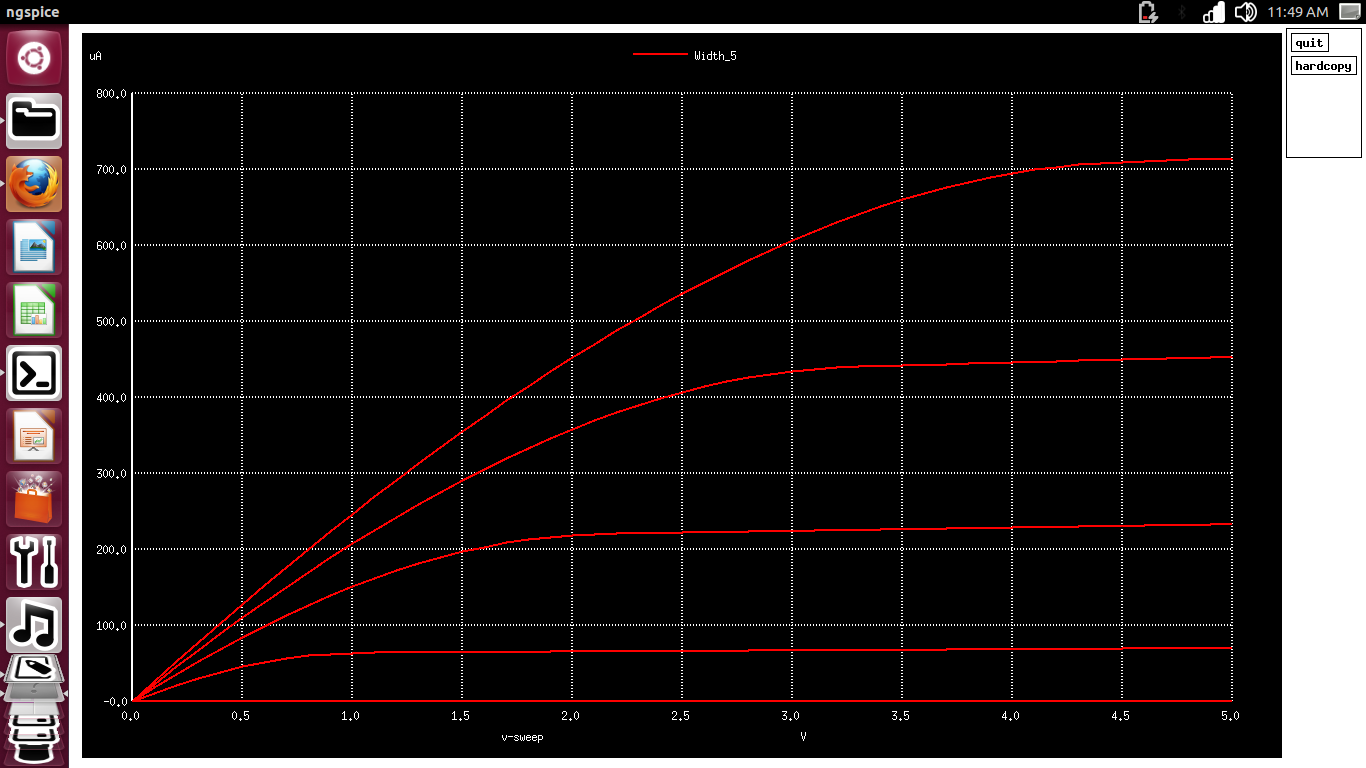
\includegraphics[scale=0.29]{Width_1c.png}
\caption[Short]{For Width = 5u}
\end{figure}
  
\vspace{3pt}
\clearpage
\textit{Conclusion:} As L increases, $I_d$ decreases. As W increases ,$I_d$ increases. As $V_{To}$ increases, $I_d$ decreases. As Lambda increases, $I_d$ increases � As VSB increases, $I_d$ decreases ( As VT increases) � As temperature increases, $I_d$ decreases 
\vspace{3pt}
\end{center}
\textbf{Parameters:}  
\\ \textbf{Voh :} Maximum output voltage when the output level is logic "1" \\ \textbf{Vol :} Minimum output voltage when the output level is logic "0"  
\\ \textbf{Vil :} Maximum input voltage which can be interpreted as logic "0"  
\\ \textbf{Vih :} Minimum input voltage which can be interpreted as logic "1"  
\\ \textbf{Rise Time:} Time taken for output voltage to change from low to high upon change in input. 
\\ \textbf{Fall Time:} Time taken for output voltage to change from high to low upon change in input.  
\\ \textbf{Noise Margin:}  NMl = Vil - Vol  NMh = Voh - Vih
\\ \textbf{Propagation Delay:} Time it takes for the output signal voltage to switch after the input signal voltage has been applied.  
\\ \textbf{Vm:} Point on the transfer characteristics curve where Vin= Vout. 



\clearpage
\begin{center}


\section{Lab 2: Study of MOS inverter with passive resistive load}
\bigskip

{\bf{Objective:}} 
Study the transfer function,Noise margin, effect on risetime, falltime ,propagation
delay, power and energy consumed of a MOS Inverter for various L, W, Load Capacitance and rise/fall time of input.\\ \vspace{2pt}
{\bf{Circuit Diagram}}
\vspace{2pt}

\begin{figure}[!ht]
\centering
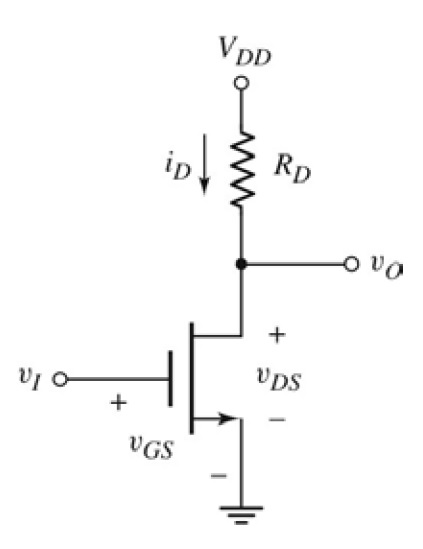
\includegraphics[scale=0.37]{nmos_inverter_with_resistive_load.jpg}
\caption[Short]{NMOS inverter with resistive load}
\end{figure}

\subsection{Varying Resistive Load and Varying Width}
\begin{lstlisting}
 
*nmos characteristics

*include model files
.include /home/vlsilab/UG_students_2014/11ec8611ec93/t14y_tsmc_025_level3.txt
*netlist
m1 out in 0 0 CMOSN l=1u w=0.5u

* Input voltage source
Vdd vdd 0 5
r0 vdd out 100
V_in in 0 dc 2.5 pulse(0 5 0 1n 1n 2n 4n)
*DC voltage source
.dc 0 5 0.000004
.tran 1n 4n

*Computing the response for various resistiv_load
.control
foreach res 100 1k 100k
alter r0 = $res
run 
end
.endc

*plotting the output for various width
.control
foreach iter 1 2 3
setplot dc$iter
plot in out
plot -Vdd#branch
setplot tran$iter
plot in out
plot -Vdd#branch
end
.endc


\end{lstlisting}

\begin{figure}[!ht]
\centering
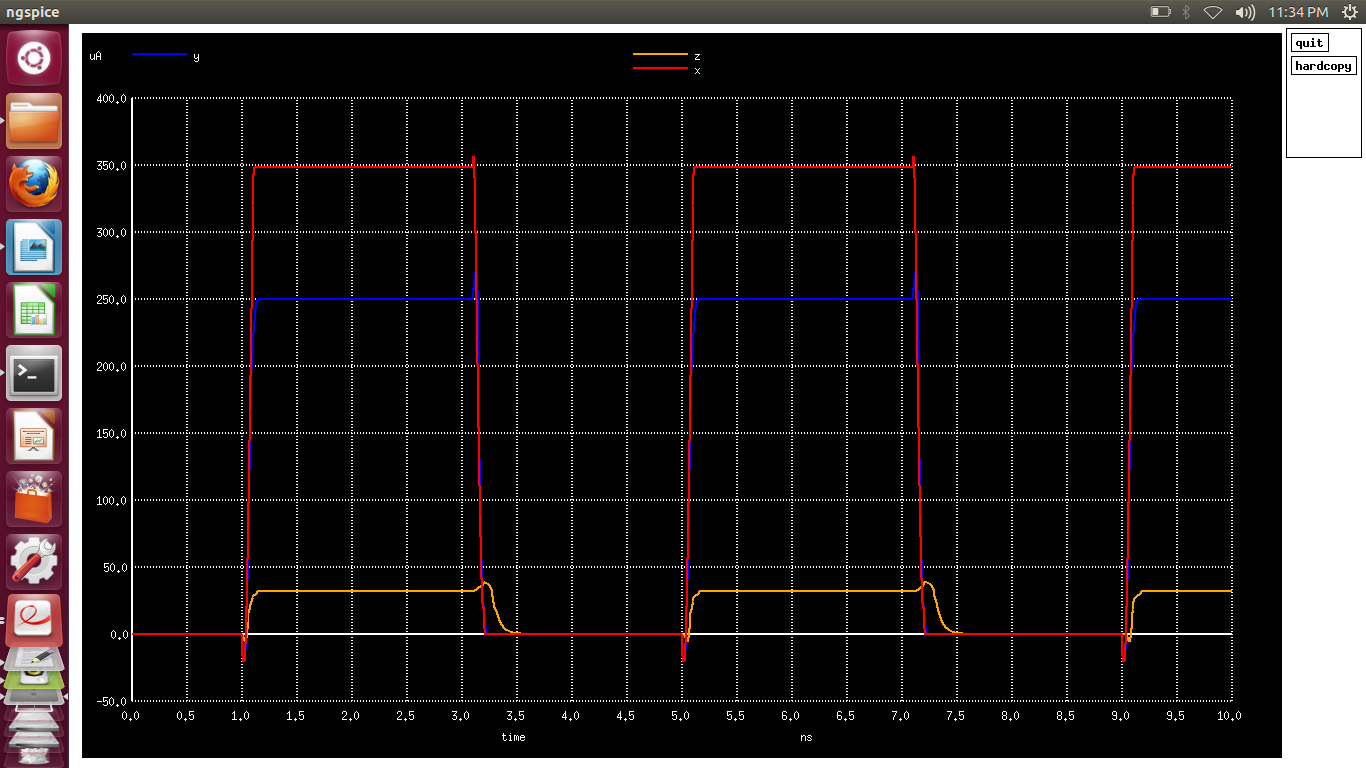
\includegraphics[scale=0.37]{lab2_current_dueto_varingR.png}
\caption[Short]{For Current due to varying Resistance}
\end{figure}
\clearpage
\begin{figure}[!ht]
\centering
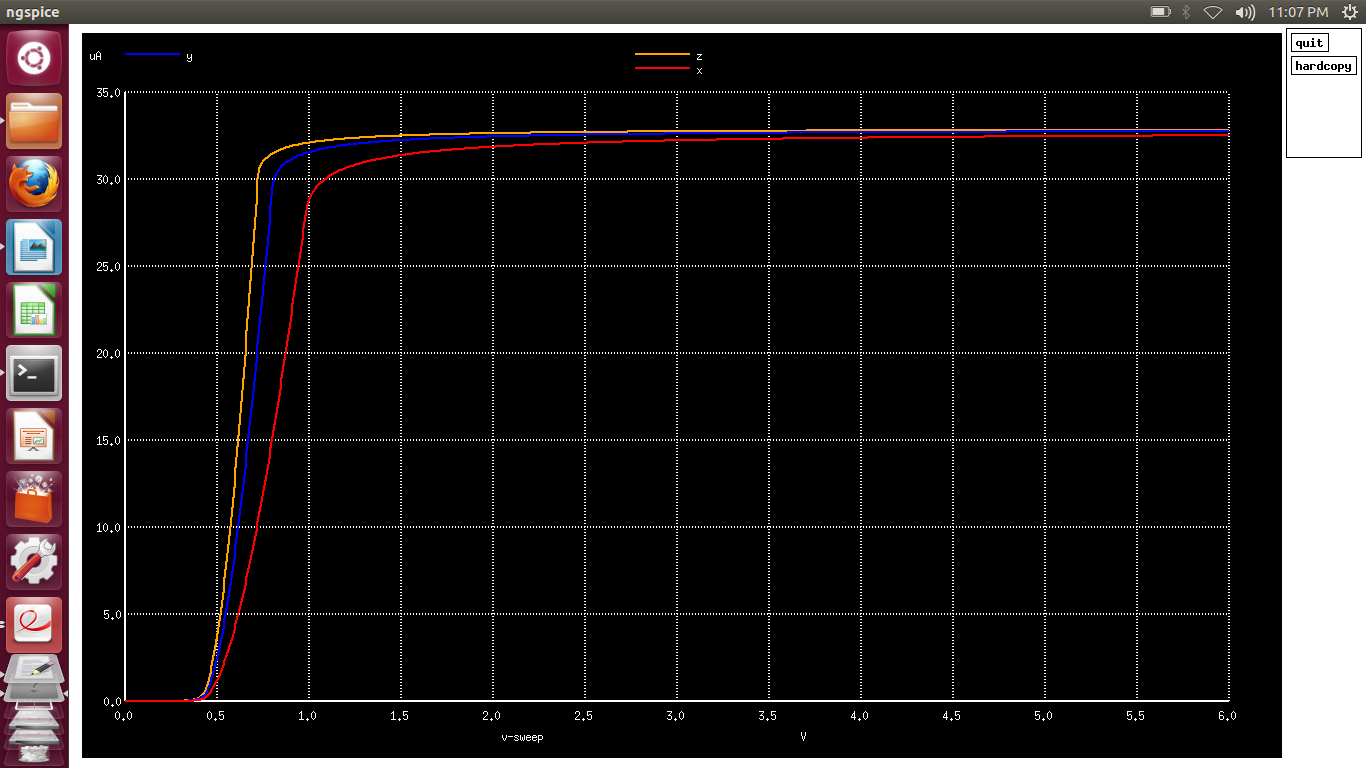
\includegraphics[scale=0.37]{lab2_DCeffect_on_current_dueto_WbyL_vary.png}
\caption[Short]{For Current due to W/L ratio variation}
\end{figure}


\subsection{Inverter DC Transfer Characteristics}
\vspace{5pt}
\begin{lstlisting}
* nmos inverter resistiv_load DC transfer function only


.include /home/krunal/VLSI_LAB/t14y_tsmc_025_level3.txt
r1 vd out 0.1k
m1 out in 0 0 CMOSN l=1u w=1u

*sources
vdd vd 0 dc 3.3 
vin in 0 dc 3.3

.dc vin 0 6 .01

* for transfer fun pic
.control
run
plot out
.endc
end
\end{lstlisting}
\begin{figure}[!ht]
\centering
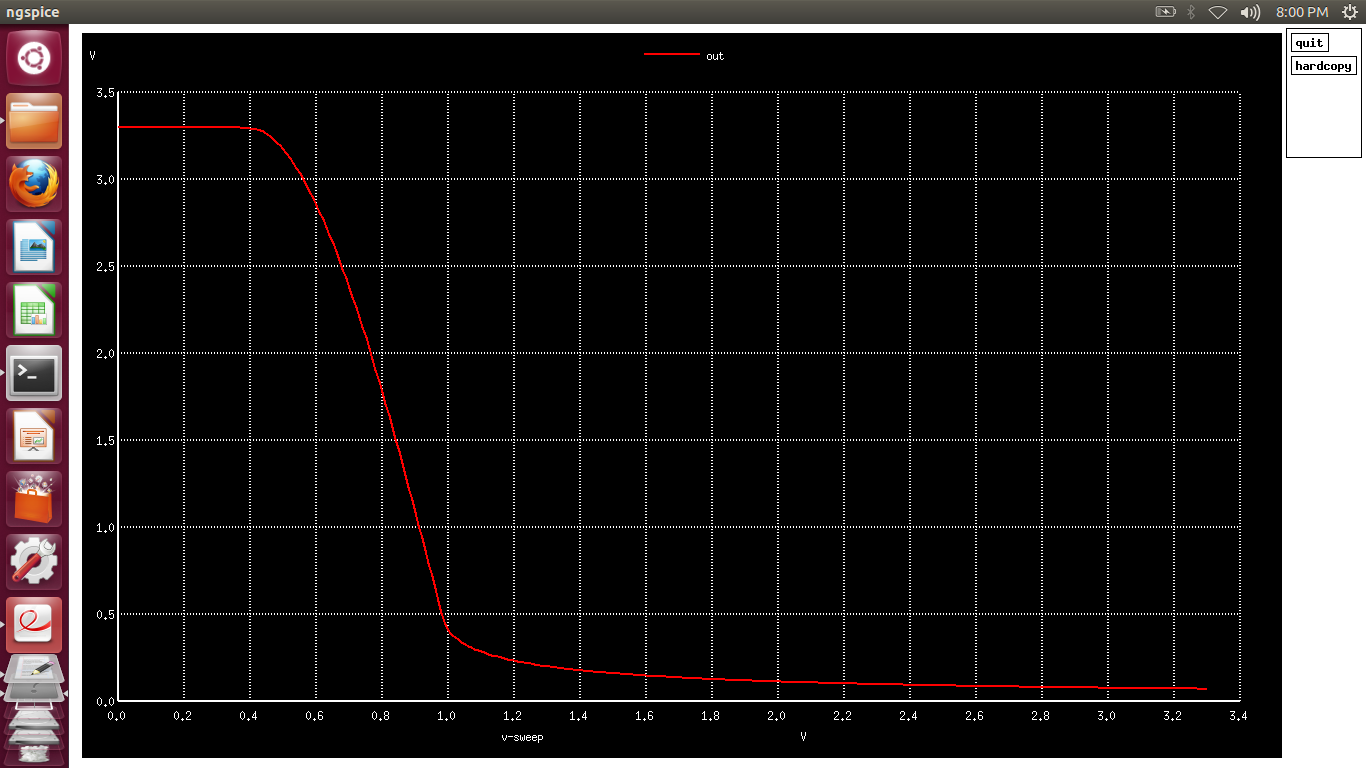
\includegraphics[scale=0.37]{lab2_lab21_transfer_char.png}

\caption[Short]{Transfer Characteristics}
\end{figure}






\begin{figure}[!ht]
\centering
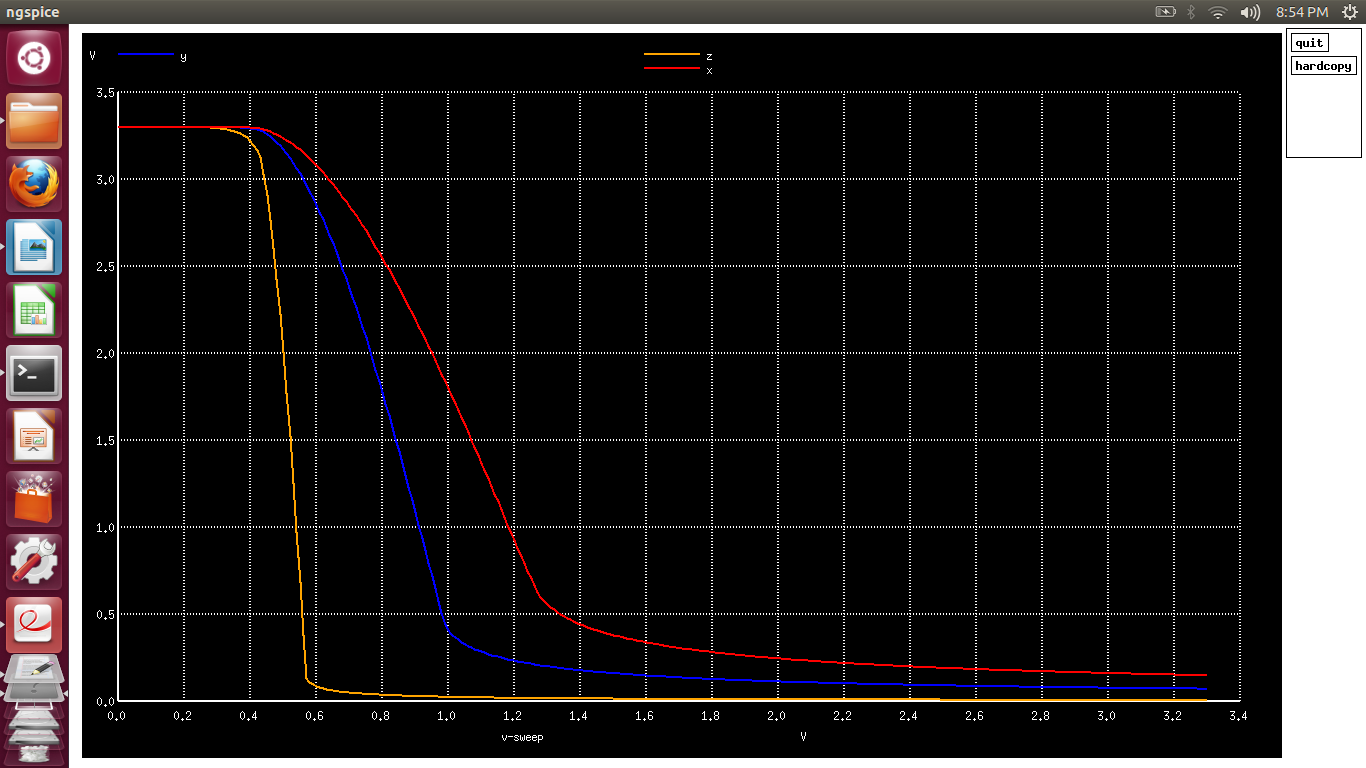
\includegraphics[scale=0.37]{lab2_lab22_varing_w_n.png}

\caption[Short]{For varying Width}
\textit{Conclusion:}  In the above figure for the VI characteristics. With increase in the value of W, the drain current increases as shown. 
\end{figure}


\begin{figure}[!ht]
\centering
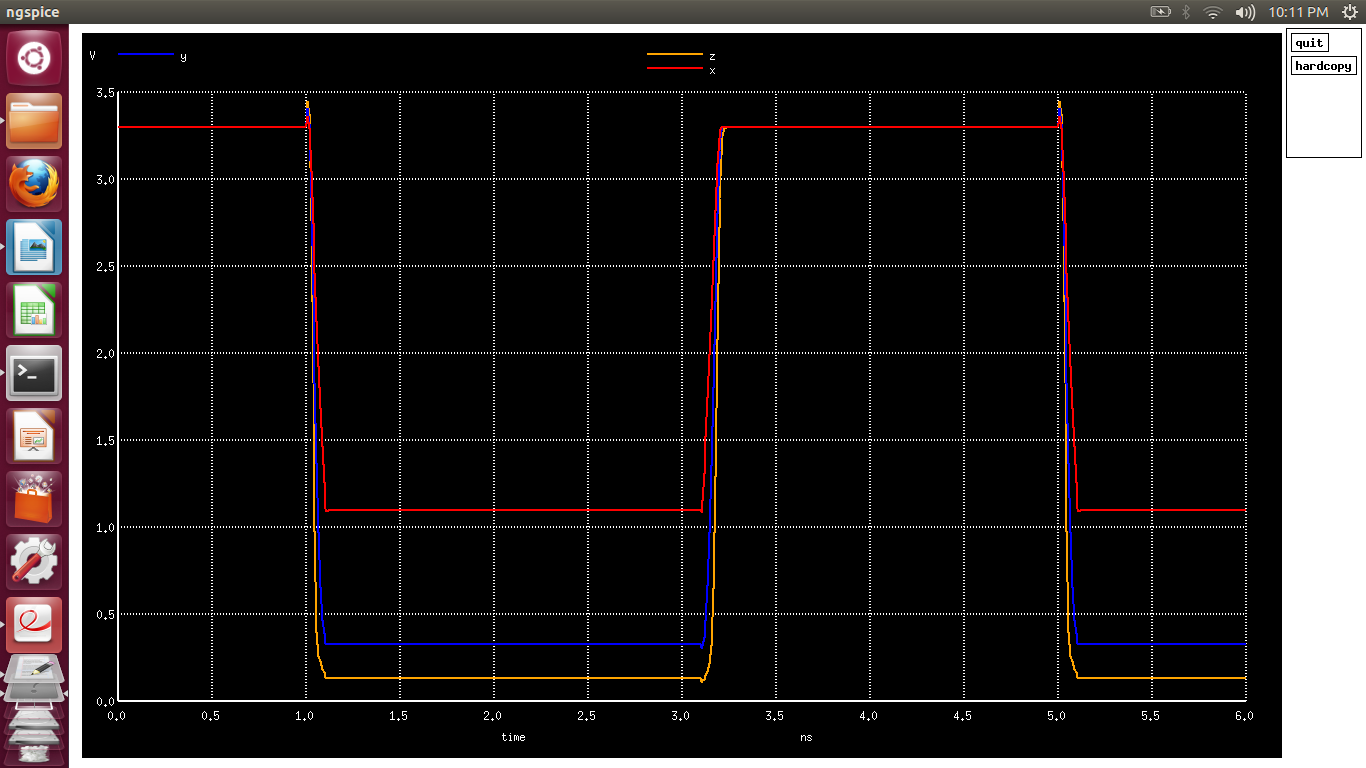
\includegraphics[scale=0.37]{lab2_pic23_tran_effect_vary_wBYL.png}
\caption[Short]{Effect on Tran on varying W/L Ratio}
\end{figure}


\begin{figure}[!ht]
\centering
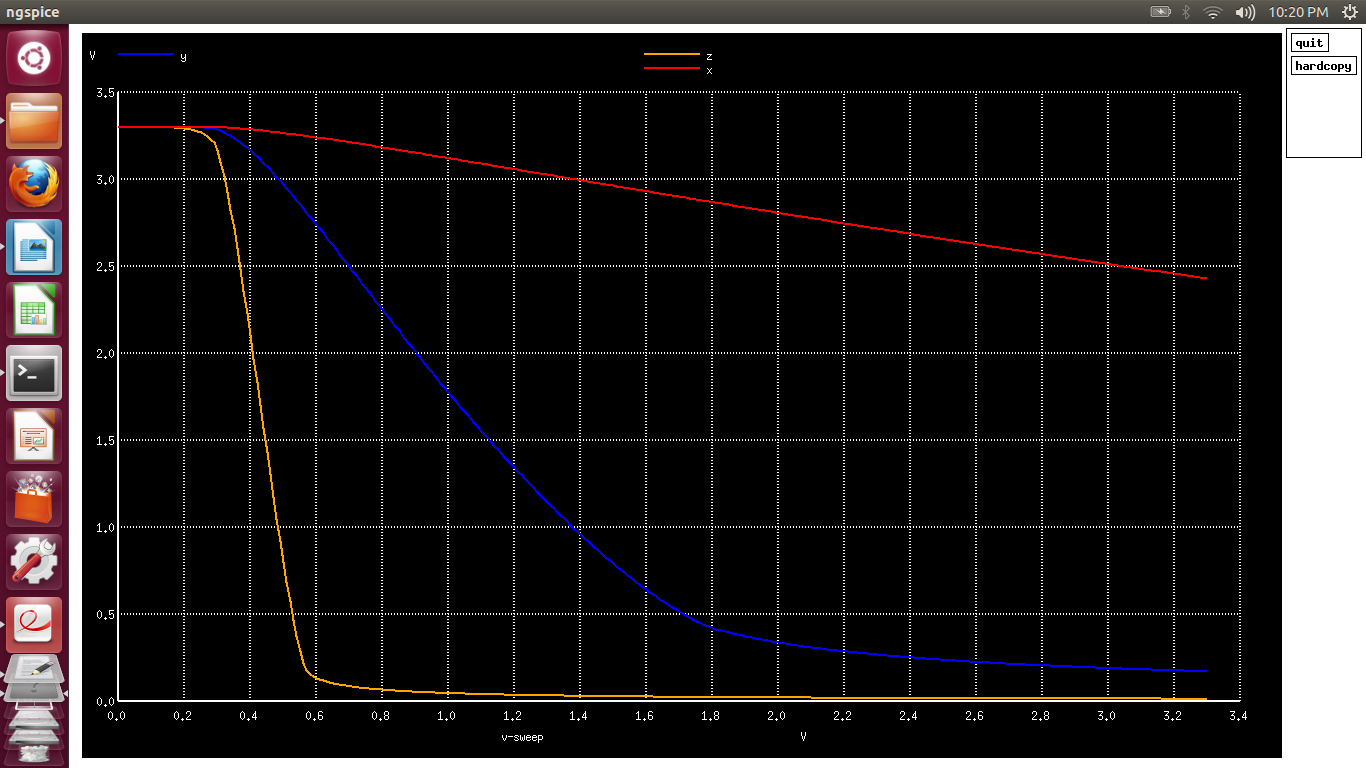
\includegraphics[scale=0.37]{lab2_pic24_effect_on_trans_char_Rvary.png}
\caption[Short]{Effect on Transfer Characteristics due to varying Resistance}
\end{figure}


\begin{figure}[!ht]
\centering
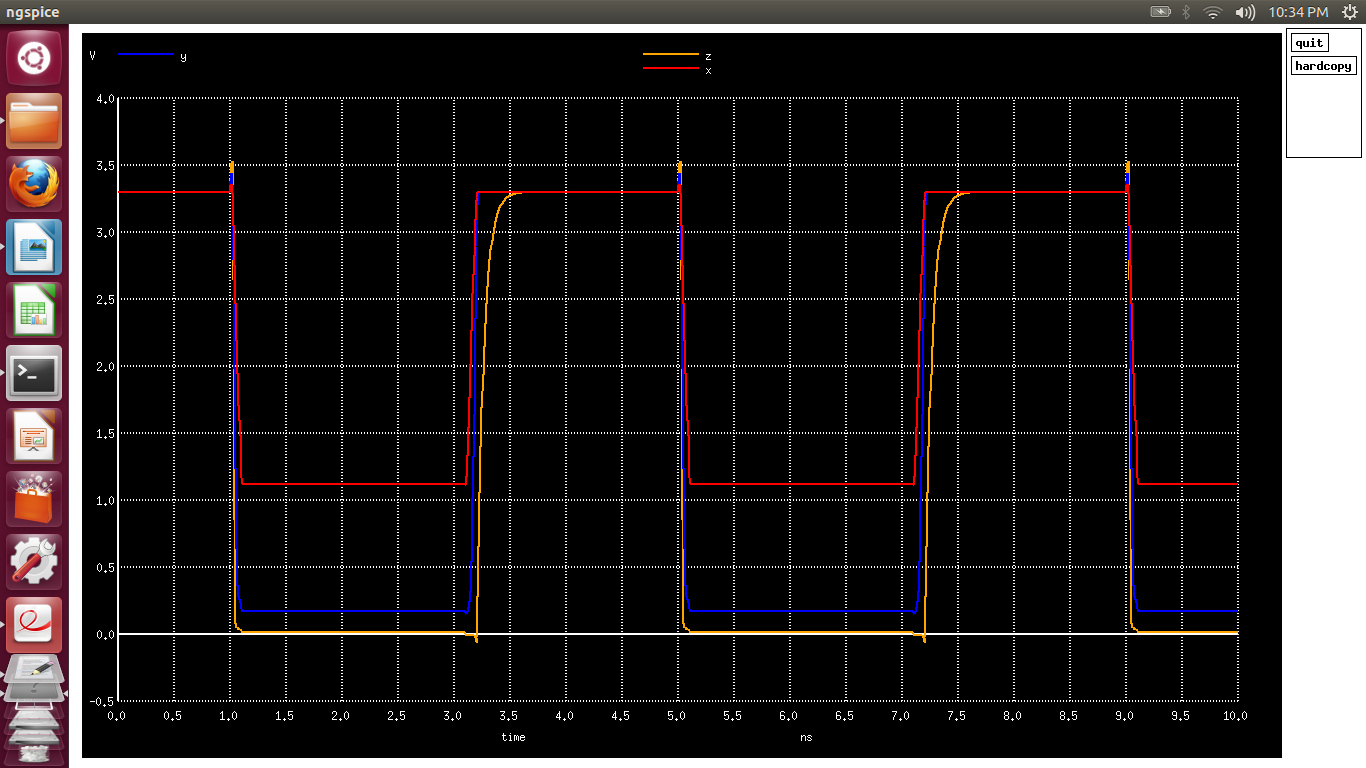
\includegraphics[scale=0.37]{lab2_pic25_effect_on_trenchar_dueto_varyR.png}
\caption[Short]{Effect on Transfer Characteristics due to varying Resistance}
\end{figure}
\clearpage

\begin{figure}[!ht]
\centering
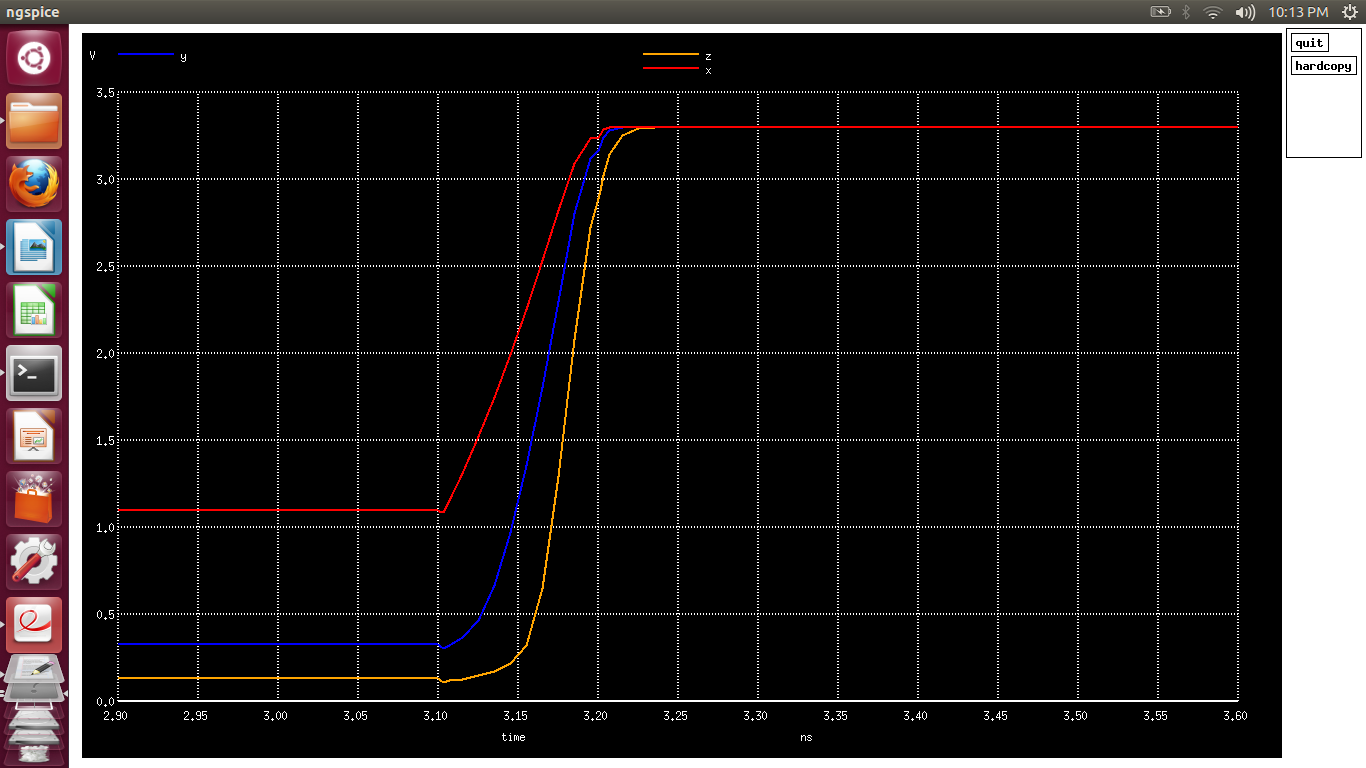
\includegraphics[scale=0.37]{lab2_pic231_rise_time_due_to_WbyL_vary.png}
\caption[Short]{Effect on Rise Time due to W/L Ratio}
\end{figure}

\begin{figure}[!ht]
\centering
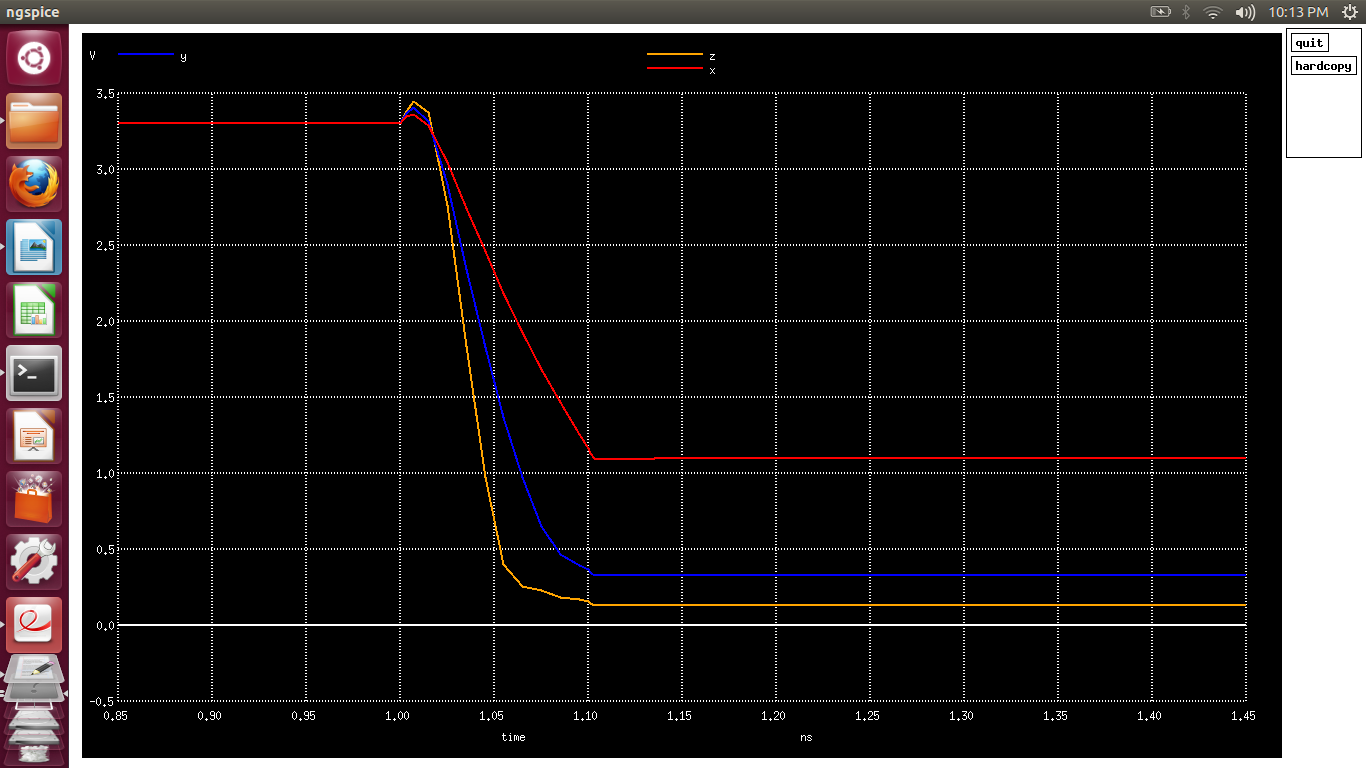
\includegraphics[scale=0.37]{lab2_pic232_fall_time_due_to_WbyL_vary.png}
\caption[Short]{effect on Fall Time due to W/L Ratio}
\end{figure}

\subsection{Power Variation}
\begin{figure}[!ht]
\centering
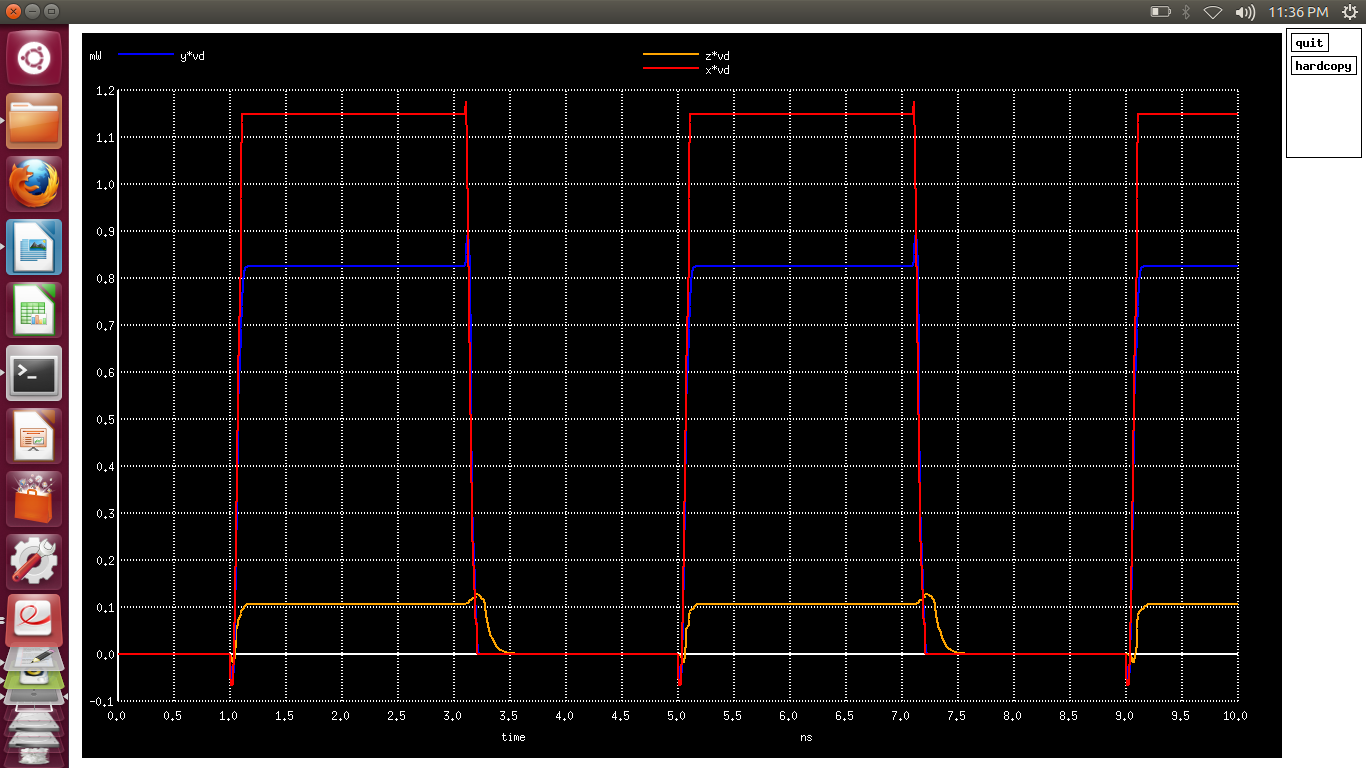
\includegraphics[scale=0.37]{lab2_power_dueto_varyR.png}
\caption[Short]{Effect on Power due to varying Resistance}
\end{figure}

\begin{figure}[!ht]
\centering
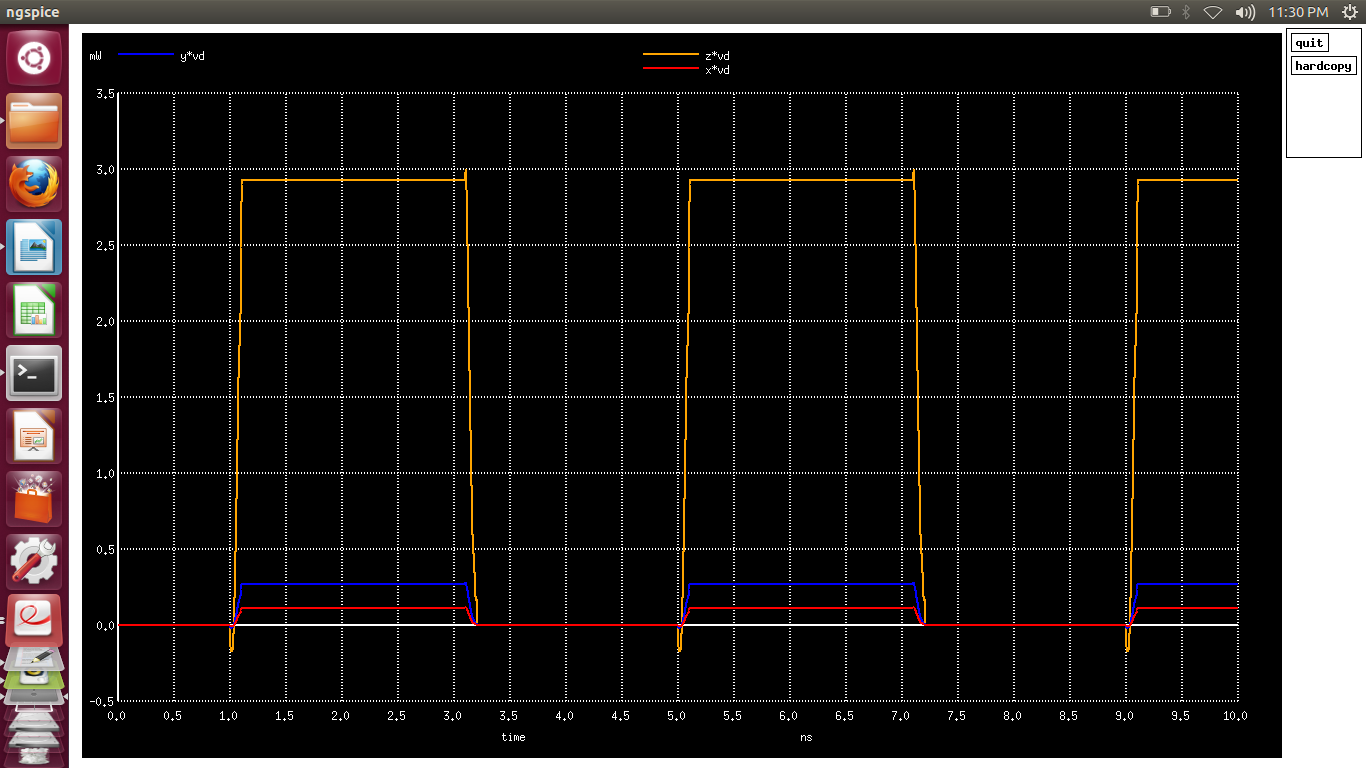
\includegraphics[scale=0.37]{lab2_power_dueto_waring_WbyL.png}
\caption[Short]{Effect on Power due to W/L Ratio}
\end{figure}
\clearpage
\subsection{Rise Time Fall Time due to Capacitance}
\begin{figure}[!ht]
\centering
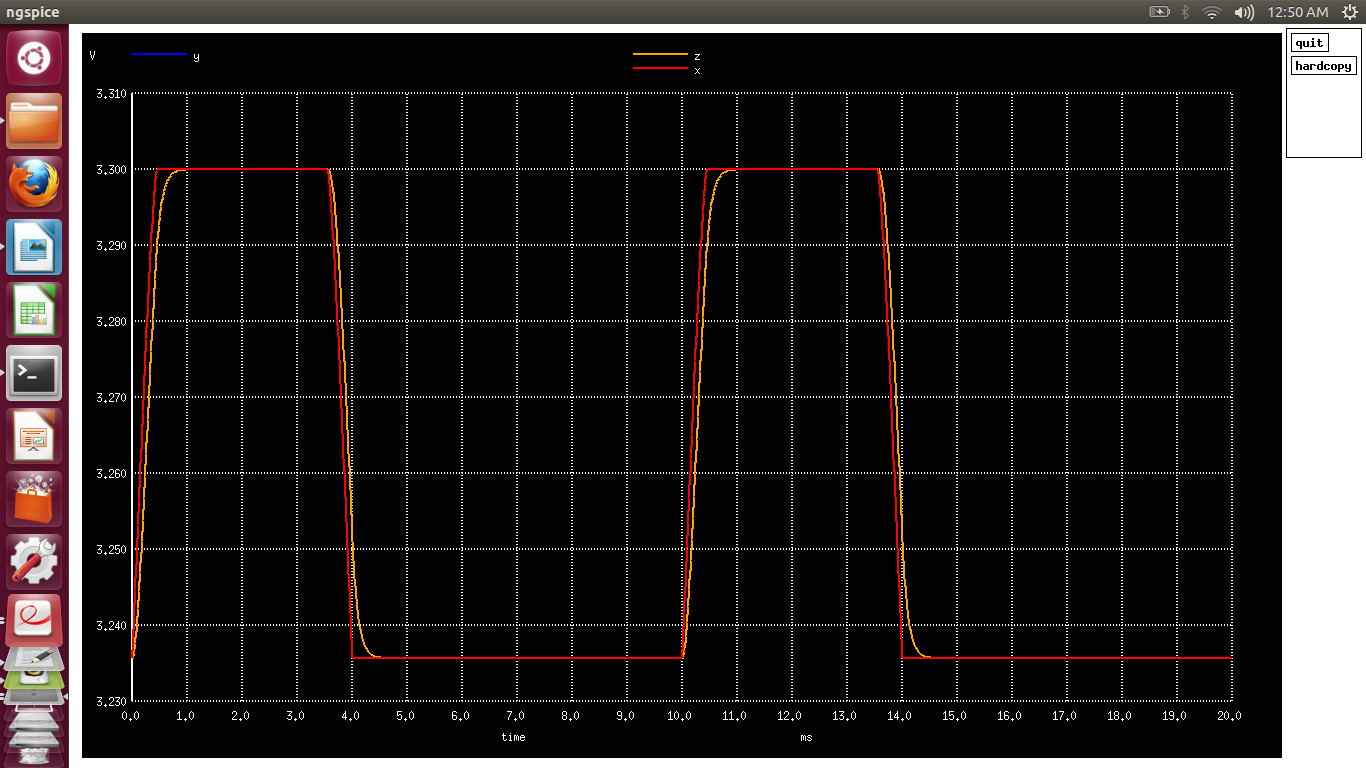
\includegraphics[scale=0.37]{lab2_risefalltime_dueto_vary_Capacitance.png}
\caption[Short]{Effect on Rise Time and Fall Time due to Varying Capacitance}
\end{figure}

\begin{figure}[!ht]
\centering
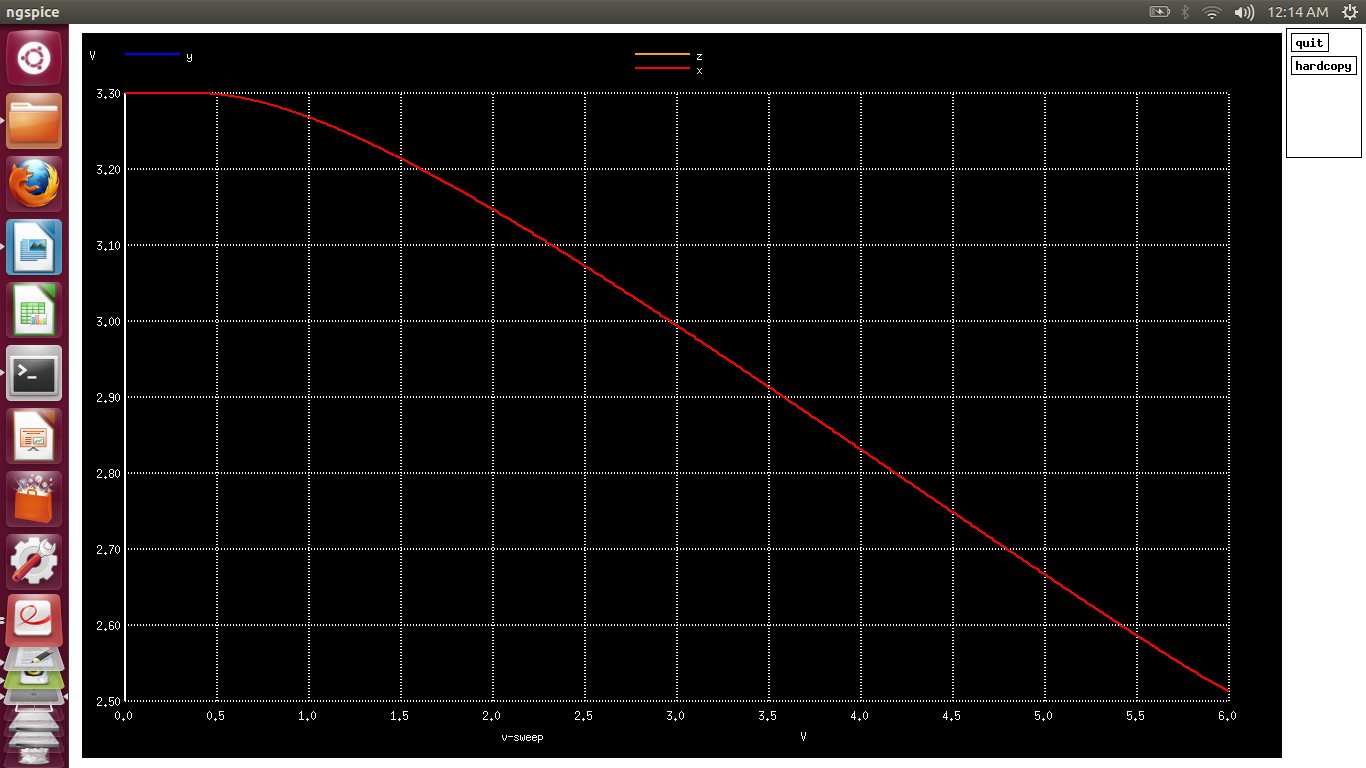
\includegraphics[scale=0.37]{lab2_dctranferchar_on_C_vary.png}
\caption[Short]{DC Transfer Characteristics due to varying Capacitance}
\end{figure}


\clearpage
\textit{Conclusion:} 
\\
As Load Resistance increases
\begin{itemize}
\item VTC shifts towards left 
\item The gain of the transition region in the VTC increases 
\item VOL decreases as R becomes larger than Resistance offered by nmos. 
\item Rise time and fall time of transient response decreases. 
\item Power consumption decreases.
\end{itemize}  
As W/L ratio increases: 
\begin{itemize}
\item VTC shifts towards left 
\item NML decreases and NMH increases 
\item TPLH increases and TPHL decreases 
\item the gain of the transition region in the VTC increases 
\item VOL decreases as Resistance offered by nmos decreases. 
\item Rise time and fall time of transient response decreases. 
\item Static and Dynamic Power consumption increases as resistance decreases.  
\end{itemize}

\clearpage


\section{Lab 3: Study of MOS inverter with active load NMOS and PMOS (pseudo NMOS load)}
\bigskip
{\bf{Objective:}}
For a MOS inverter with active load NMOS and PMOS (pseudo NMOS load),Study the transfer function, noise margin, effect on rise time, fall time, propagation delay,
power and energy consumed by a NMOS inverter with NMOS, PMOS load for various L,W of the pull-up and pulldown transistors and to determine the power and
energy consumed with non-ideal step input.

\underline{\bf{Circuit Diagram}}\\
\vspace{2pt}

\begin{figure}[!ht]
\centering
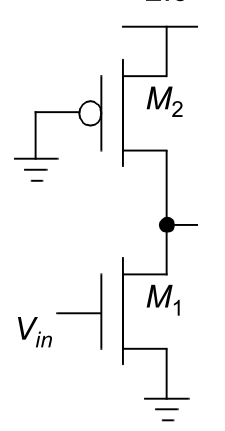
\includegraphics[scale=0.6]{pseudo.png}
\caption[Short]{Pseudo Nmos}
\end{figure}
\subsection{Pseudo Nmos load inverter DC transfer characteristics}

\begin{lstlisting}
.include /home/krunal/VLSI_LAB/t14y_tsmc_025_level3.txt

m0 vd out 0 5 CMOSP l=2u w=1u
m1 out in 0 0 CMOSN l=2u w=1u	

*sources
vdd vd 0 dc 5 
vin in 0 dc 5 

.dc vin 0 5 .001

*for transfer char pic
.control
run
plot out
end
.endc

\end{lstlisting}
\begin{figure}[!ht]
\centering
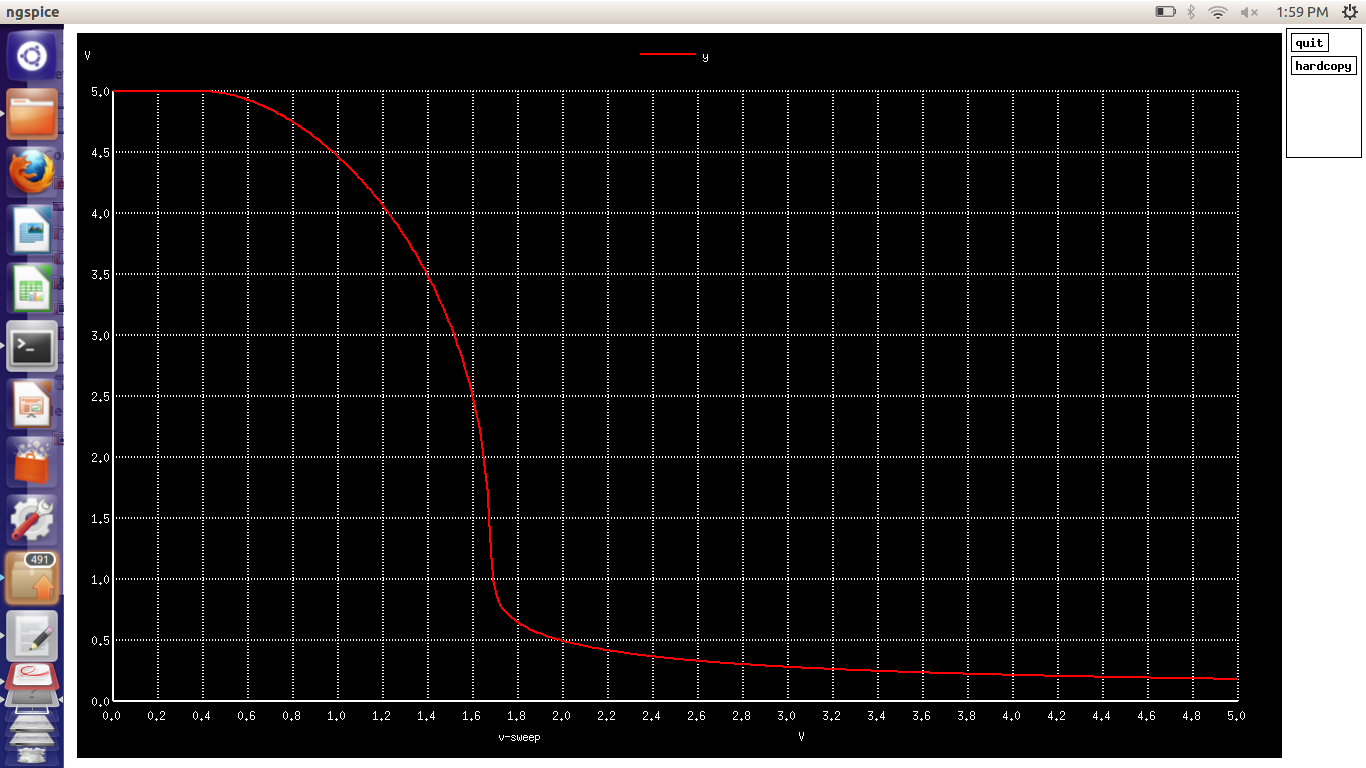
\includegraphics[scale=0.37]{lab3_pic3_1_transfer_char_only.png}
\caption[Short]{Transfer Characteristics}
\end{figure}

\textit{Conclusion:}
VOH can never be equal to VDD as NMOS can pull up to only VDD-VT.
\\ As W/L of NMOS LOAD decreases 
\subsection{Transient Response}

\begin{lstlisting}

.include /home/krunal/VLSI_LAB/t14y_tsmc_025_level3.txt

m0 out 0 vd 5 CMOSP l=1u w=1u
m1 out in 0 0 CMOSN l=1u w=1u

*sources
vdd vd 0 dc 5 
vin in 0 dc 5 pulse(5 0 1u 10u 10u 2m 4m)

*for transfer fun pic
.control
tran .01m 10m
run
plot out,in
end
.endc

\end{lstlisting}
\begin{figure}[!ht]
\centering
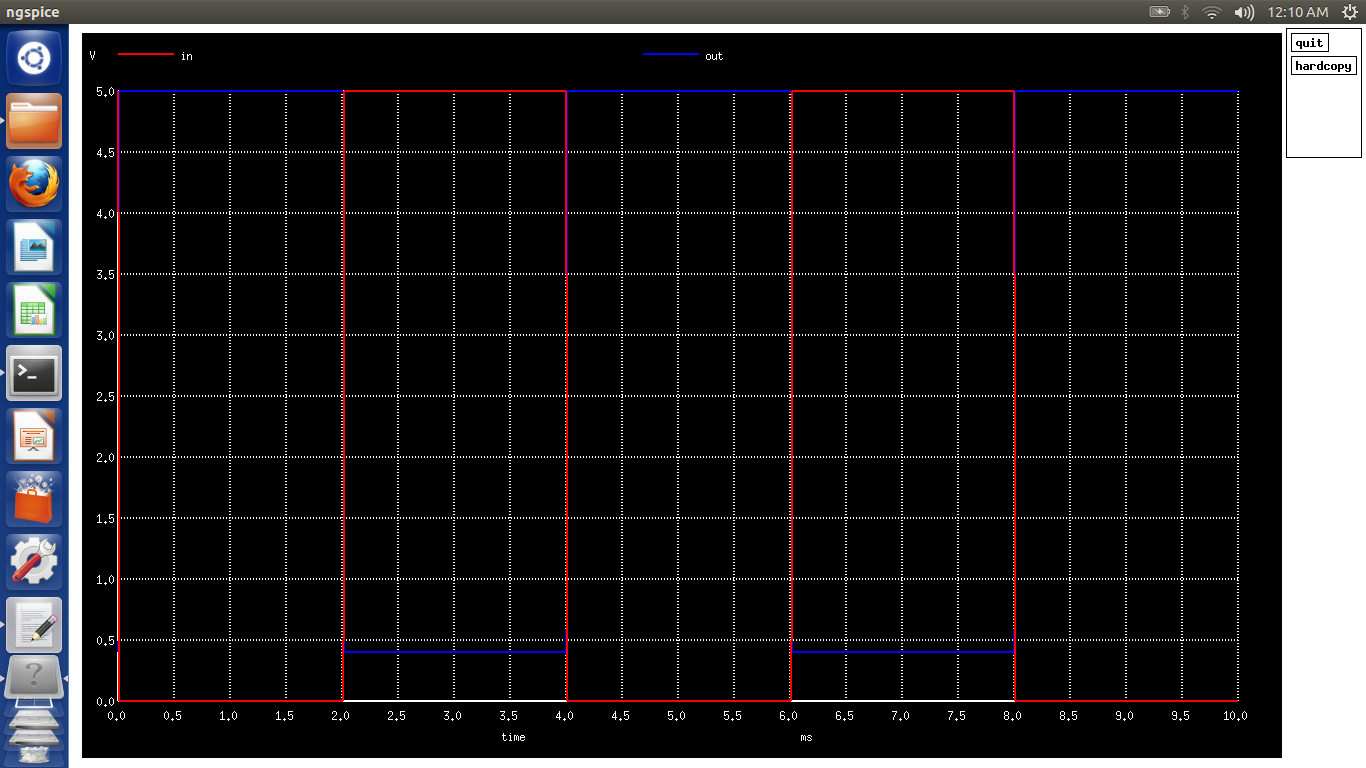
\includegraphics[scale=0.37]{lab3_pic3_2_transient_response.png}

\caption[Short]{Transient Response}
\end{figure}
\subsection{Transfer characteristics due to varying width of driver}

\begin{lstlisting}

.include /home/krunal/VLSI_LAB/t14y_tsmc_025_level3.txt

m0 vd 0 out 5 CMOSP l=1u w=1u  *LOAD 
m1 out in 0 0 CMOSN l=1u w=1u  *Driver

*sources
vdd vd 0 dc 5 
vin in 0 dc 5 

.dc vin 0 5 .01

*varing W/L ratio
.control
foreach wid 1u 2u 4u
alter m1 w = $wid
run 
end
.endc


*plotting the output for various w of load
.control
foreach iter 1 2 3
setplot dc$iter
end
.endc

.control
let x= dc1.out
let y= dc2.out
let z= dc3.out
plot x,y,z
end
.endc

\end{lstlisting}

\begin{figure}[!ht]
\centering
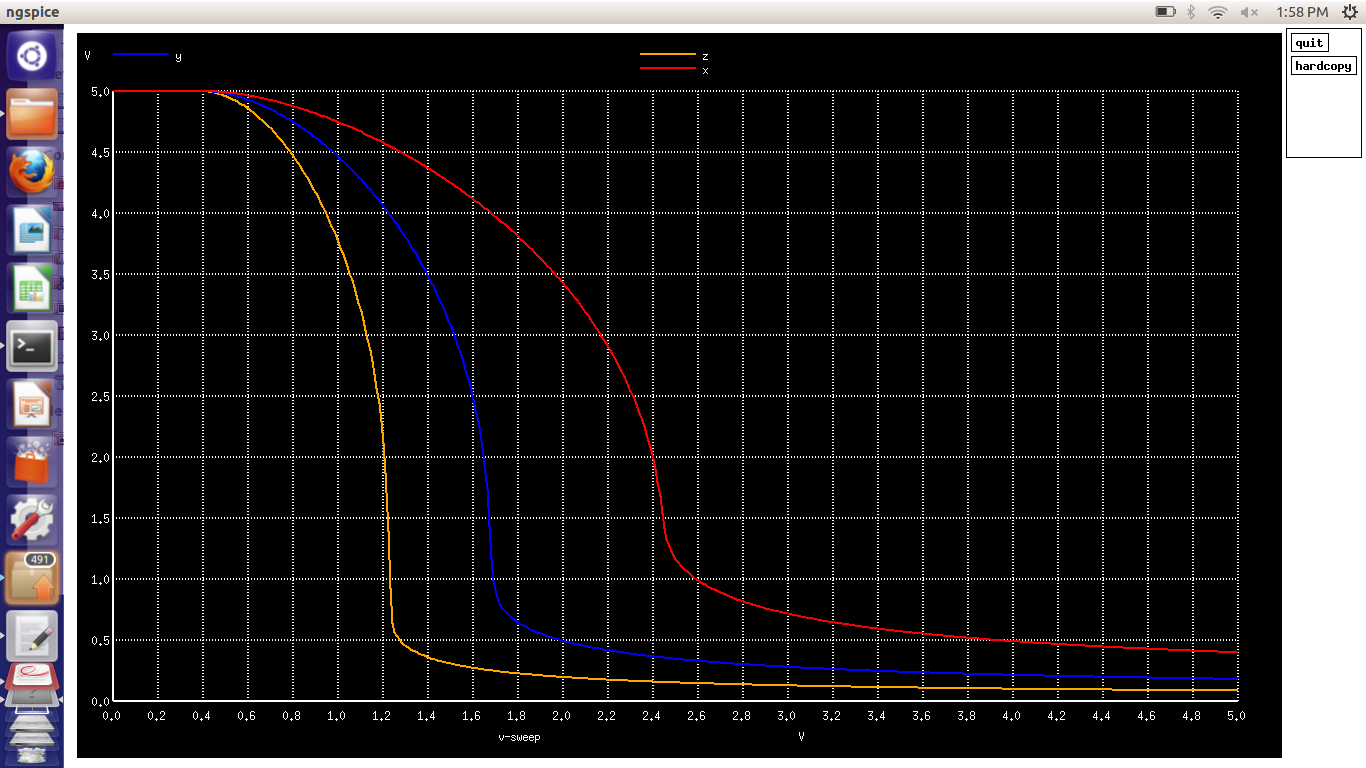
\includegraphics[scale=0.37]{lab3_pic3_3__trans_char_dueto_varing_w_of_driver.png}

\caption[Short]{Transfer Characteristics due to varying of W of the Driver}
\end{figure}
\subsection{Transient Response due to varying width of driver}

\begin{lstlisting}

.include /home/krunal/VLSI_LAB/t14y_tsmc_025_level3.txt

m0 vd 0 out 5 CMOSP l=2u w=1u  *LOAD 
m1 out in 0 0 CMOSN l=2u w=1u	 *Driver

*sources
vdd vd 0 dc 5 
vin in 0 dc 5 pulse(0 5 10n 10u 10u 1m 2m)

*.dc vin 0 5 .01

*varing W/L ratio
.control
foreach wid .5u .8u 1.5u
alter m1 w = $wid
tran 0.01m 5m
end
.endc


*plotting the output for various w of load
.control
foreach iter 1 2 3
setplot tran$iter
end
.endc

.control
let x= tran1.out
let y= tran2.out
let z= tran3.out
plot x,y,z
end
.endc
\end{lstlisting}

\begin{figure}[!ht]
\centering
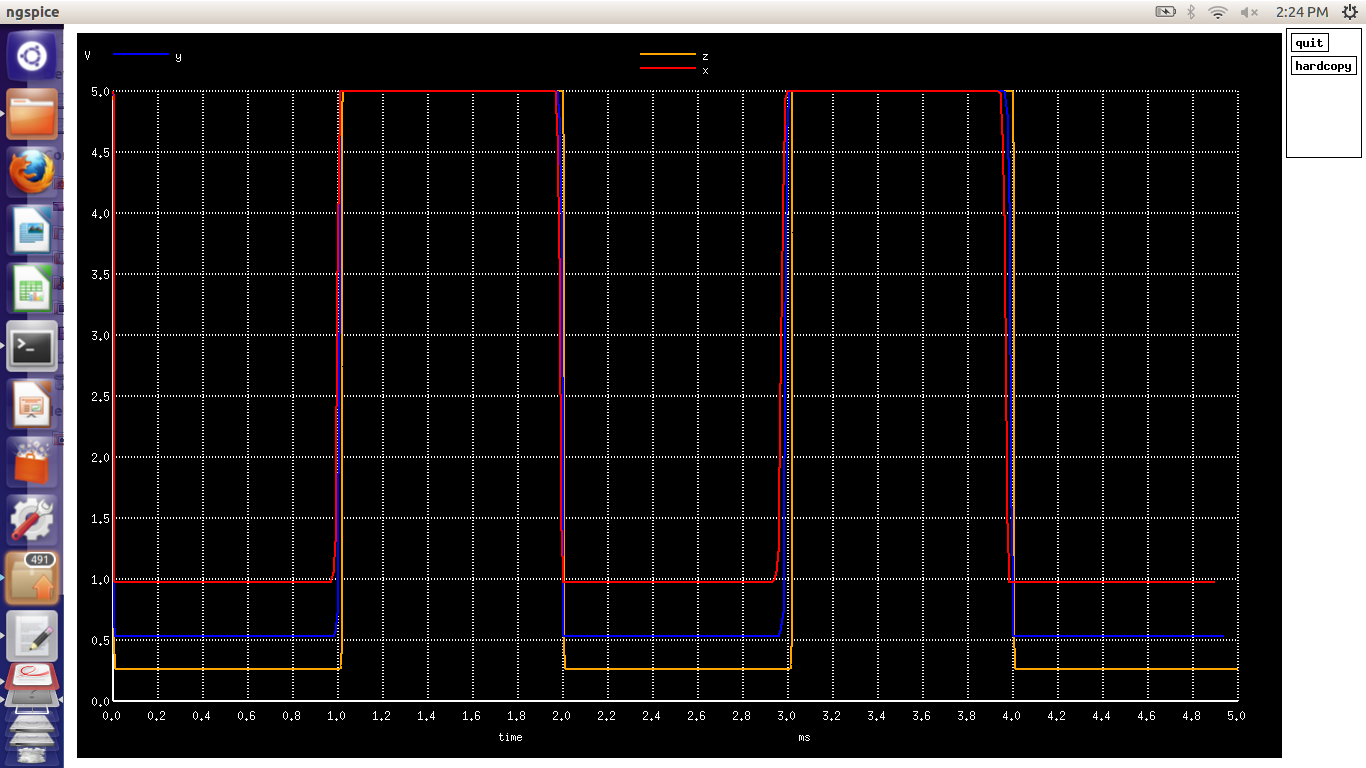
\includegraphics[scale=0.37]{lab3_pic3_4_transient_dueto_varing_Wof_driver.png}
\caption[Short]{Transient Response after varying W of the Driver}
\end{figure}

\subsection{Transfer Function and Transient Response due to varying length of driver}
\begin{lstlisting}

.include /home/krunal/VLSI_LAB/t14y_tsmc_025_level3.txt

m0 vd 0 out 5 CMOSP l=2u w=1u 
m1 out in 0 0 CMOSN l=2u w=1u	

*sources
vdd vd 0 dc 5 
vin in 0 dc 5 pulse(0 5 10n 10u 10u 1m 2m)

*varing L of driver
.control
foreach len .5u 2u 4u
alter m1 l = $len
run
tran 0.01m 5m
end
.endc


*plotting the output for various w of load
.control
foreach iter 1 2 3
setplot tran$iter
end
.endc

.control
let x= tran1.out
let y= tran2.out
let z= tran3.out
plot x,y,z
end
.endc

\end{lstlisting}

\begin{figure}[!ht]
\centering
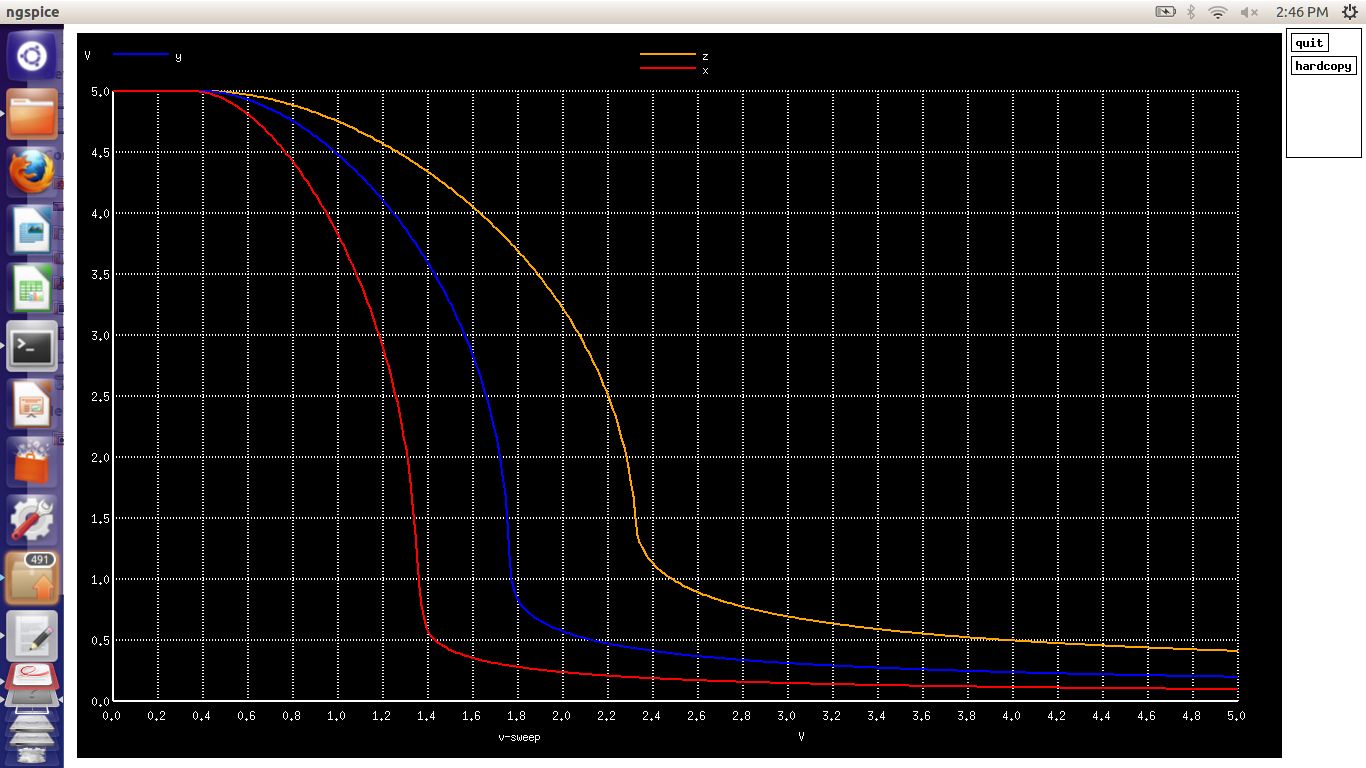
\includegraphics[scale=0.31]{lab_3pic3_5_transfer_fun_dueto_varing_Lof_driver.png}
\caption[Short]{Transfer characteristics due to varying the length of the Driver}
\end{figure}

\begin{figure}[!ht]
\centering
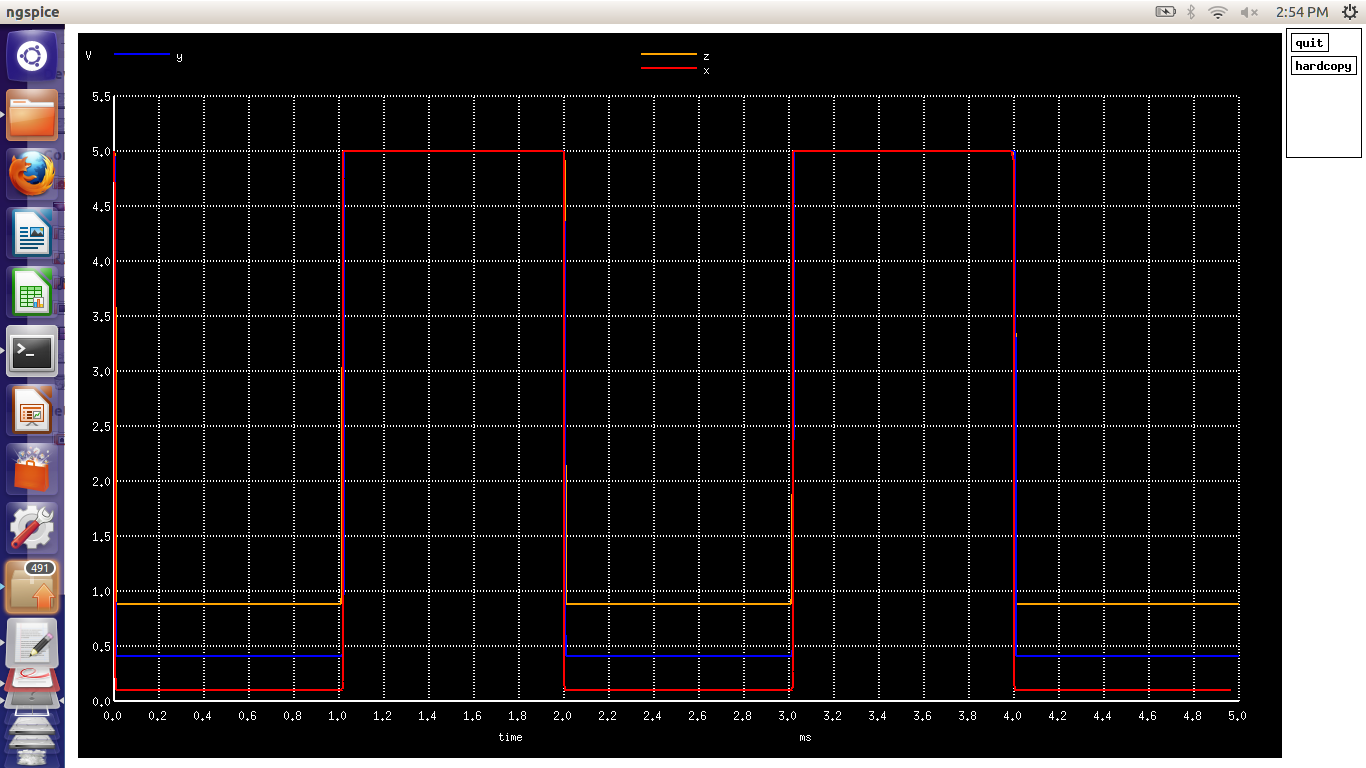
\includegraphics[scale=0.37]{lab3_pic3_52_transient_dueto_varing_Lof_driver.png}
\caption[Short]{Transient Response due to varying the Length of the driver}
\end{figure}

\clearpage
\subsection{Transfer Characteristics due to varying width of load}
\begin{lstlisting}

.include /home/krunal/VLSI_LAB/t14y_tsmc_025_level3.txt

m0 vd 0 out 5 CMOSP l=1u w=1u  *LOAD 
m1 out in 0 0 CMOSN l=1u w=1u  *Driver

*sources
vdd vd 0 dc 5 
vin in 0 dc 5 pulse

.dc vin 0 5 .01

*varing W of load pmos ratio
.control
foreach wid .125u .25u 2.5u
alter m0 w = $wid
run 
end
.endc


*plotting the output for various w of load
.control
foreach iter 1 2 3
setplot dc$iter
end
.endc

.control
let x= dc1.out
let y= dc2.out
let z= dc3.out
plot x,y,z
end
.endc
\end{lstlisting}
\clearpage
\begin{figure}[!ht]
\centering
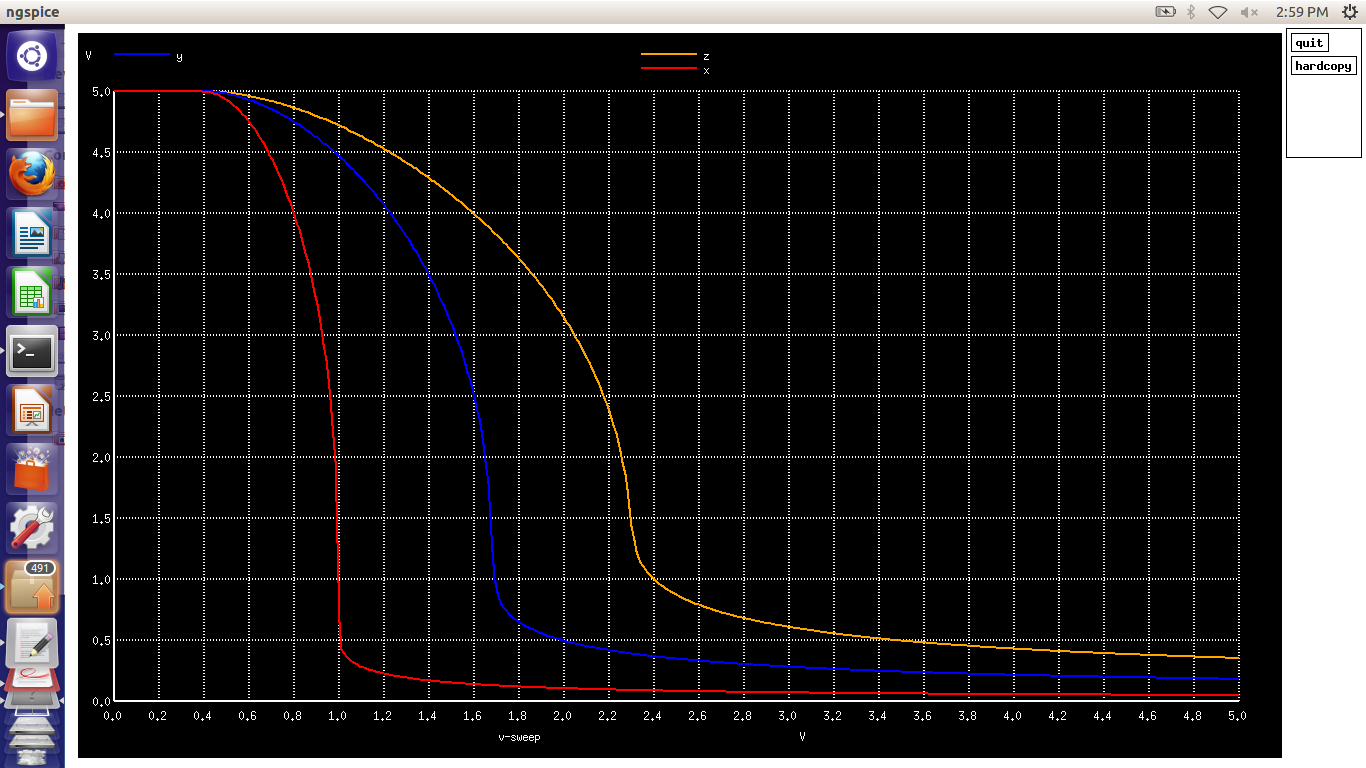
\includegraphics[scale=0.37]{lab3_pic3_6_transfer_fun_dueto_varing_Wof_load.png}
\caption[Short]{Transfer Function on varying the Width of the Load}
\end{figure}

\subsection{Transient Response on varying length of load}
\begin{lstlisting}

.include /home/krunal/VLSI_LAB/t14y_tsmc_025_level3.txt

m0 vd 0 out 5 CMOSP l=1u w=1u  *LOAD 
m1 out in 0 0 CMOSN l=1u w=1u  *Driver

*sources
vdd vd 0 dc 5 
vin in 0 dc 5 pulse(0 5 0 0 0 .5m 1m)

*varing W/L ratio
.control
foreach len 1u 2u 5u
alter m0 l = $len
run 
tran 0.01m 2m
end
.endc


*plotting the output for various L of load
.control
foreach iter 1 2 3
setplot trans$iter
end
.endc

.control
let x= tran1.out
let y= tran2.out
let z= tran3.out
plot x,y,z
end
.endc

\end{lstlisting}

\begin{figure}[!ht]
\centering
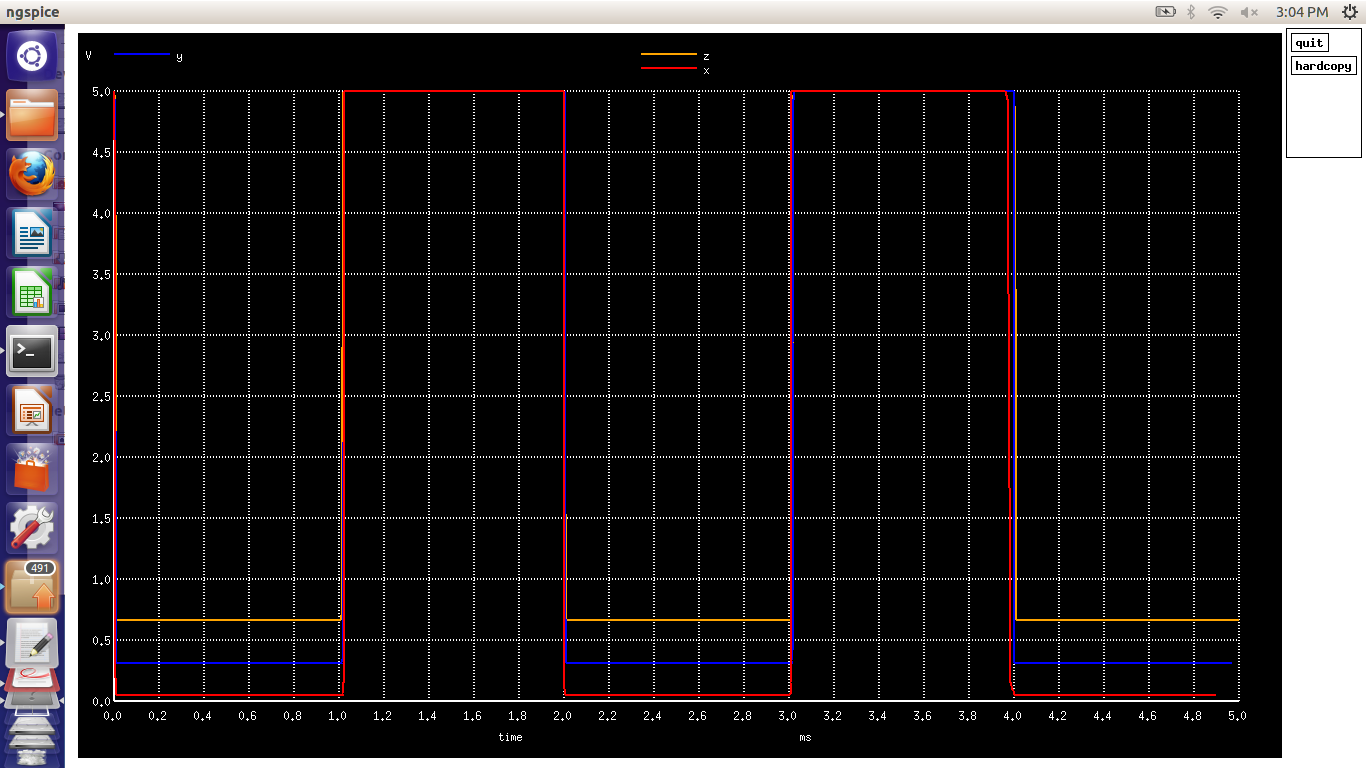
\includegraphics[scale=0.37]{lab3_pic3_6_transient_dueto_varing_Lof_load.png}

\caption[Short]{Transient Response due to varying the Length of the Load}
\end{figure}

\begin{figure}[!ht]
\centering
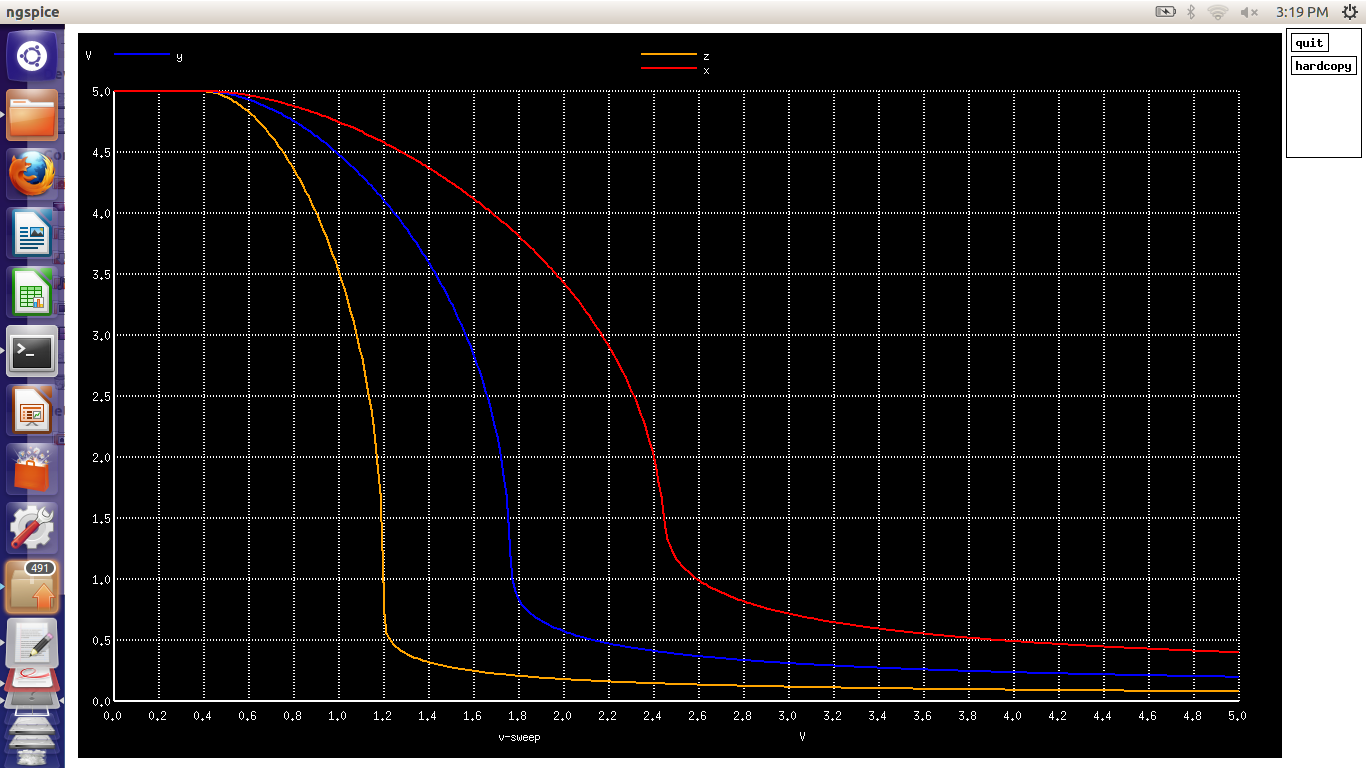
\includegraphics[scale=0.37]{lab3_pic3_7_transfer_fun_dueto_varing_Lof_load.png}

\caption[Short]{Transfer Characteristics due to varying the Length of the load}
\end{figure}

\begin{figure}[!ht]
\centering
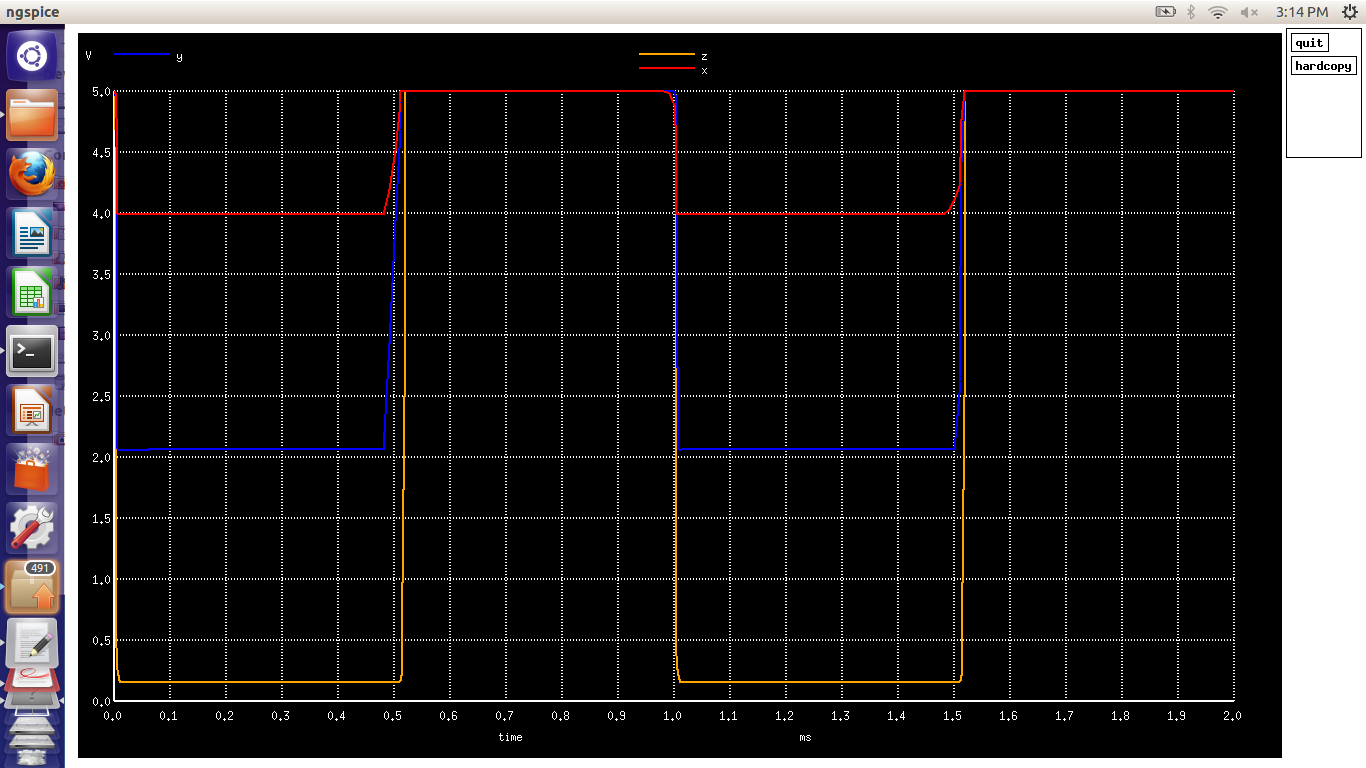
\includegraphics[scale=0.37]{lab3_pic3_7_transient_duto_varing_Lof_load.png}

\caption[Short]{Transient Response due to varying the length of the load}
\end{figure}
\clearpage
\newpage
\subsection{Conclusion:}
As W/L of NMOS increases • 
\begin{itemize}
\item VTC shifts towards left • 
\item The gain of the transition region in the VTC increases. • 
\item NML decreases and NMH increases • 
\item TPLH increases and TPHL decreases • 
\item VOL decreases as R becomes smaller than Resistance offered by pmos. • 
\item Power Dissipation Increases as R is smaller and also energy consumed per    transition increases. • 
\item Rise/Fall time reduces.
\end{itemize}  
As W/L of PMOS LOAD decreases • 
\begin{itemize}
\item VTC shifts towards left • 
\item the gain of the transition region in the VTC increases • 
\item NML decreases and NMH increases • 
\item TPLH increases and TPHL decreases • 
\item VOL decreases as Resistance offered by pmos increases. • 
\item Static and Dynamic Power Dissipation decreases as R is larger and also energy consumed per transition decreases. • 
\item Rise/Fall time reduces.
\end{itemize}  
As Load Capacitance increases, Rise/Fall time of output increases and Energy consumed per transition increases. 
\\Also Static power increases. As input rise time and fall time increases TPHL and TPLH increases 

\clearpage

\subsection{Study of inverter with NMOS load}
\vspace{5pt}
{\bf{Objective:}} 
For a  inverter with NMOS load,study
the transfer function, effect on rise time, fall time, propagation delay,
power and energy consumed by  inverter with variation in  L,W 
of the pull-up and pulldown transistors and to determine the power and energy consumed with non-ideal step input.\\
\underline{\bf{Circuit Diagram}}\\
\vspace{2pt}
\begin{figure}[!ht]
\centering
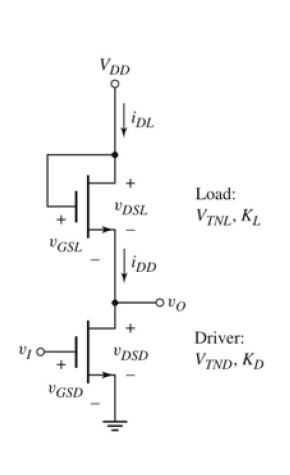
\includegraphics[scale=0.37]{nmos_inverter_with_enhancement_load.jpg}

\caption[Short]{Nmos Inverter with enhancement load}
\end{figure}

\subsection{Transient Response due to varying length of load}
\begin{lstlisting}

.include /home/krunal/VLSI_LAB/t14y_tsmc_025_level3.txt

m0 vd vd out 0 CMOSN l=1u w=.3u 
m1 out in 0 0 CMOSN l=1u w=5u	
c1 out 0 1p

*sources
vdd vd 0 dc 5 
vin in 0 dc 5  pulse(0 5 0 0 0 2u 4u)

*varing W of driver
.control
foreach len 1u 2u 5u
alter m0 l = $len
tran .01u 10u
run 
end
.endc


*plotting the output for various length of load
.control
foreach iter 1 2 3
setplot tran$iter
end
.endc

*ploting graph for transient out
.control
let x= tran1.out
let y= tran2.out
let z= tran3.out
plot x,y,z
end
.endc

\end{lstlisting}


\begin{figure}[!ht]
\centering
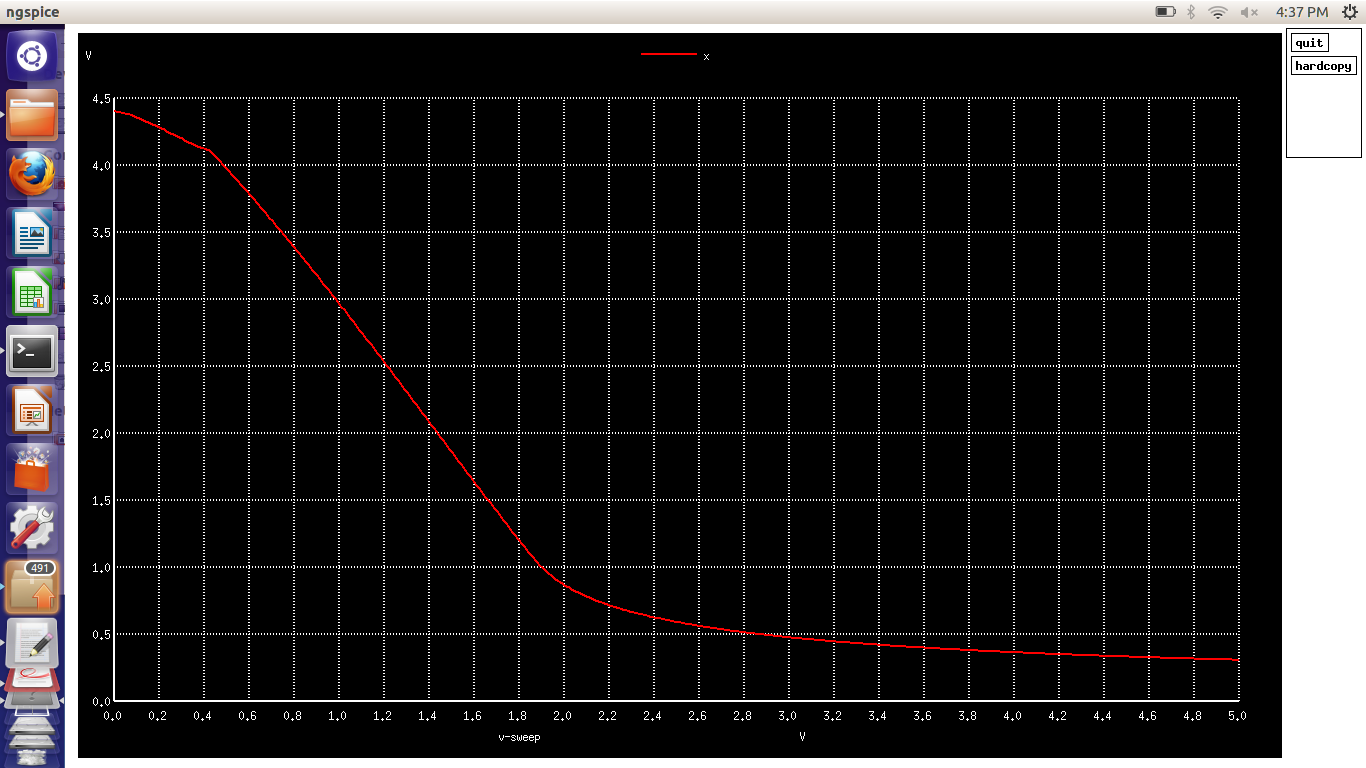
\includegraphics[scale=0.37]{lab4_pic4_1_trsnfer_fun_only.png}

\caption[Short]{Transfer function of  inverter with NMOS load}
\end{figure}

\begin{figure}[!ht]
\centering
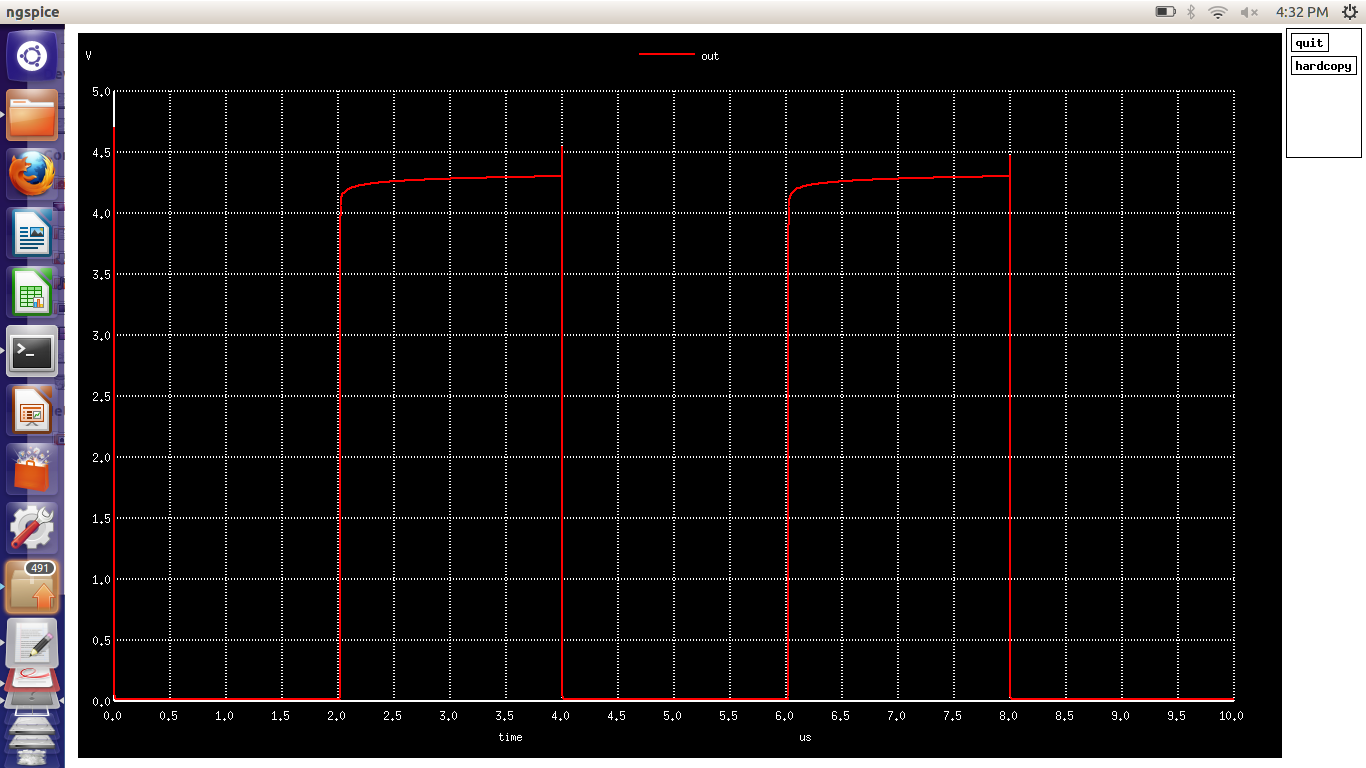
\includegraphics[scale=0.37]{lab4_pic4_2_transient_out.png}

\caption[Short]{Transient output}
\end{figure}

\clearpage
\subsection{Transient Response due to varying width of load}
\begin{lstlisting}
*  inverter with  NMOS load
*transient response only

.include /home/krunal/VLSI_LAB/t14y_tsmc_025_level3.txt

m2 vd vd out 0 cmosn l=1u w=.1u
m1 out in 0 0 cmosn l=1u w=5u

*sources
vdd vd 0 dc 5 
vin in 0 dc 5 pulse(0 5 0 0 0 2u 4u)

.control
tran .01u 10u
run
plot out,in
.endc
\end{lstlisting}

\begin{figure}[!ht]
\centering
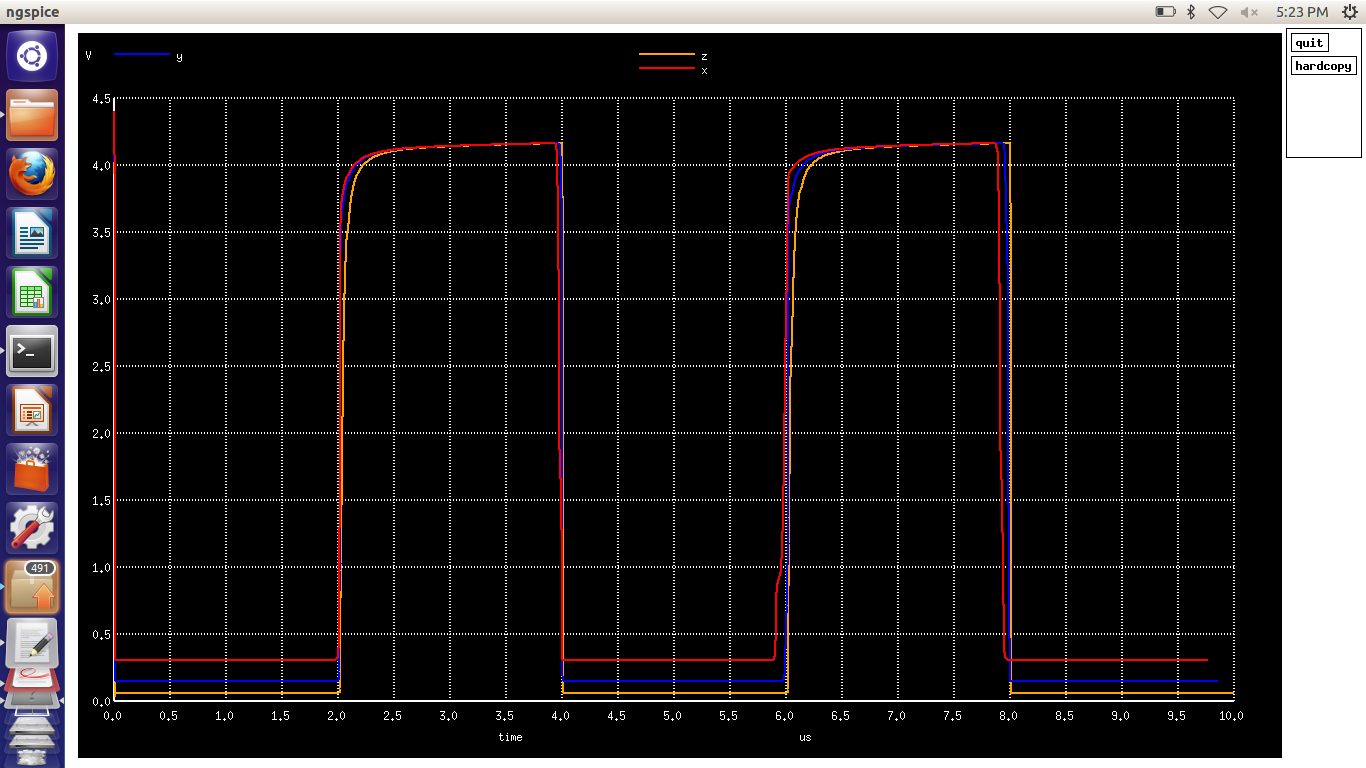
\includegraphics[scale=0.37]{lab4_pic4_2_transient_dueto_varing_Wof_deiver.png}

\caption[Short]{Transient Response due to varying the Width of the Driver}
\end{figure}
\clearpage



\begin{figure}[!ht]
\centering
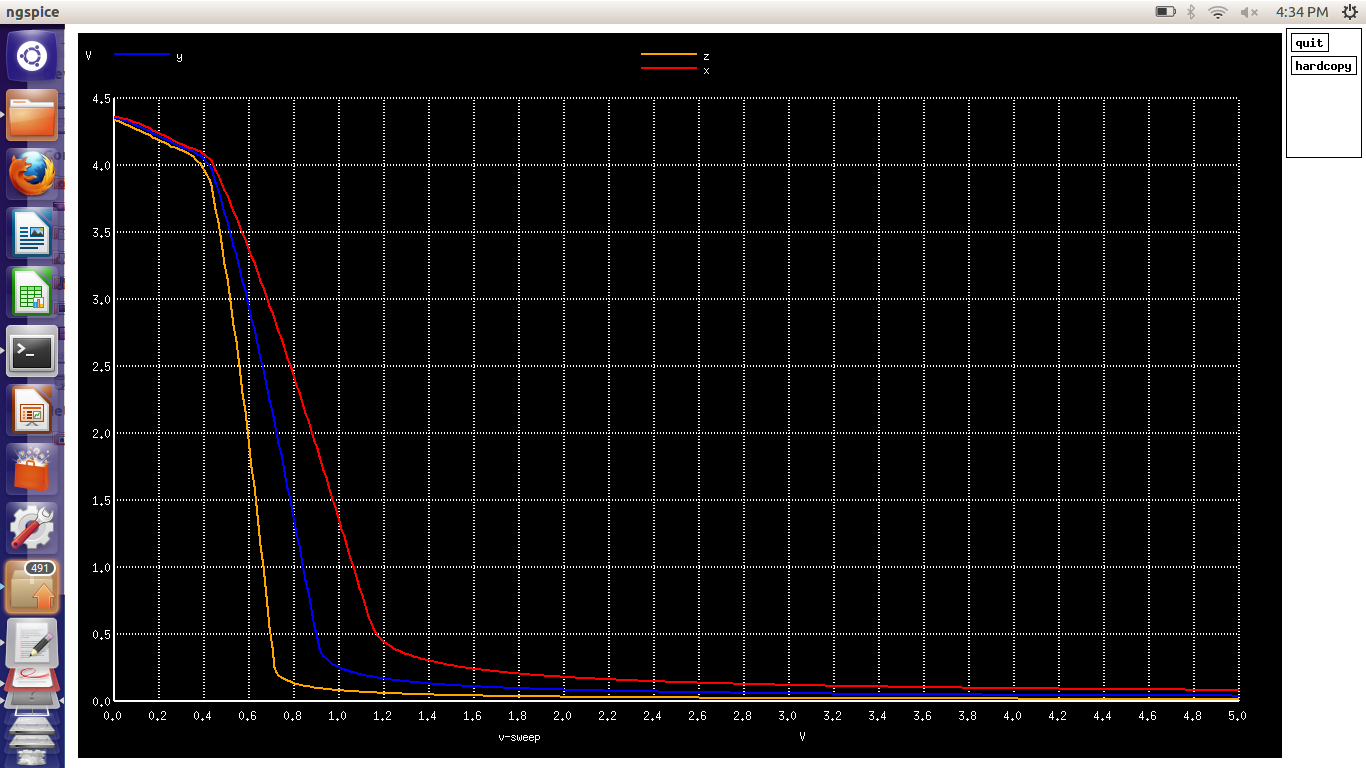
\includegraphics[scale=0.37]{lab4_pic4_3_transfer_dueto_varing_Wof_driver.png}

\caption[Short]{Transfer due to varying the width of driver}
\end{figure}

\begin{figure}[!ht]
\centering
\includegraphics[scale=0.37]{lab4_pic4_4_2_transient_dueto_varing_Lof_driver.png}

\caption[Short]{Transient Response due to varying the length of the Driver}
\end{figure}

\begin{figure}[!ht]
\centering
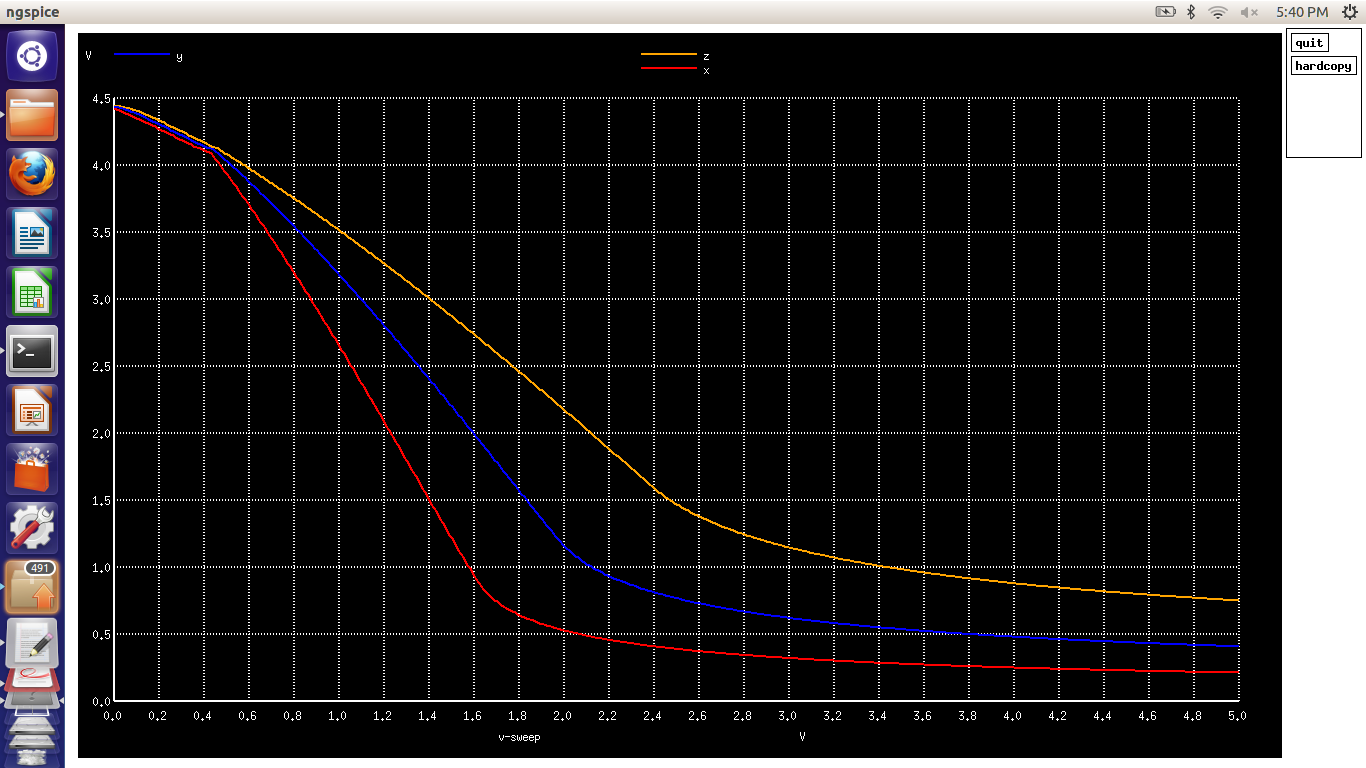
\includegraphics[scale=0.37]{lab4_pic4_4_tranfer_char_dueto_varing_Lof_driver.png}

\caption[Short]{Transfer Characteristics due to varying the length of the driver}
\end{figure}

\subsection{Transient Response due to varying length of driver}
\begin{lstlisting}
.include /home/krunal/VLSI_LAB/VINAY/t14y_tsmc_025_level3.txt

m0 vd vd out 0 CMOSN l=1u w=1u  *LOAD 
m1 out in 0 0 CMOSN l=1u w=5u	*Driver

*sources
vdd vd 0 dc 5
vin in 0 dc 5 pulse(0 5 0 0 0 2u 4u)

*.dc vin 0 5 .01

*varing W/L ratio
.control
foreach len 1u .2u .4u
alter m1 l = $len
tran .01u 15u
run
end
.endc


*plotting the output for various length of  driver
.control
foreach iter 1 2 3
setplot tran$iter
end
.endc

\end{lstlisting}
\begin{figure}[!ht]
\centering
\includegraphics[scale=0.37]{lab4_pic4_5_1_transfer_fun_dueto_varing_Lof_loadnmos.png}

\caption[Short]{Transfer function due to varying the length of the load - nmos}
\end{figure}

\clearpage


\subsection{Static Power due to variation in length}
\begin{figure}[!ht]
\centering
\includegraphics[scale=0.37]{lab4_pic4_5_2_static_power_dueto_varing_Lof_loadnmos.png}

\caption[Short]{Static Power due to varying the Length of load nmos}
\end{figure}

\begin{figure}[!ht]
\centering
\includegraphics[scale=0.37]{lab4_pic4_5_3_transient_dueto_varing_Lof_loadnmos.png}

\caption[Short]{Transient Response due to varying the length of the load}
\end{figure}

\subsection{Dynamic Power due to varying the length of load nmos}
\begin{figure}[!ht]
\centering
\includegraphics[scale=0.37]{lab4_pic4_5_4_dynamic_power_dueto_varing_Lof_loadnmos.png}

\caption[Short]{Dynamic Power due to varying the Length of load nmos}
\end{figure}

\begin{figure}[!ht]
\centering
\includegraphics[scale=0.37]{lab4_pic4_6_1_transfer_char_dueto_varing_Wof_loadnmos.png}

\caption[Short]{Transient Characteristics due to varying the Width of load- nmos}
\end{figure}

\subsection{Static Power due to varying Width of load}
\begin{figure}[!ht]
\centering
\includegraphics[scale=0.37]{lab4_pic4_6_2_static_power_dueto_varing_Wof_loadnmos.png}
\caption[Short]{Static Power due to varying W of the load nmos}
\end{figure}

\begin{figure}[!ht]
\centering
\includegraphics[scale=0.37]{lab4_pic4_6_5_transient_dueto_varing_Wof_loadnmos.png}

\caption[Short]{Transient Response due to varying the Width of the load nmos}
\end{figure}

\subsection{Dynamic Power due to varying width of load nmos}
\begin{figure}[!ht]
\centering
\includegraphics[scale=0.37]{lab4_pic4_6_6_dynamic_power_dueto_varing_Wof_loadnmos.png}

\caption[Short]{Dynamic Power due to varying the Width of the load nmos}
\end{figure}

\begin{figure}[!ht]
\centering
\includegraphics[scale=0.37]{lab4_pic4_10_dynamic_power_dueto_varing_Wof_driver.png}

\caption[Short]{Dynamic Power due to varying the Width of the driver}
\end{figure}
\clearpage
\subsection{Static Power due to varying Width of Driver}
\begin{figure}[!ht]
\centering
\includegraphics[scale=0.37]{lab4_pic4_11_static_power_dueto_varing_wof_driver.png}

\caption[Short]{Static Power due to varying the Width of the Driver}
\end{figure}

\begin{figure}[!ht]
\centering
\includegraphics[scale=0.37]{lab4_pic4_12_dynamic_power_dueto_varing_Lof_driver.png}

\caption[Short]{Dynamic Power due to varying the Length of the Driver}
\end{figure}
\clearpage
\textit{Conclusion:}
VOH can never be equal to VDD as NMOS can pull up to only VDD-VT.
\\ As W/L of NMOS LOAD decreases 
\begin{itemize}
\item VTC Shifts towards left 
\item The gain of the transition region in the VTC increases 
\item NML decreases and NMH increases 
\item TPLH increases and TPHL decreases 
\item VOL decreases as Resistance offered by nmos increases. • 
\item Power Dissipation decreases as R is larger and also energy consumed per transition decreases. • 
\item Rise/Fall time of output reduces.
\end{itemize}
As W/L of NMOS increases • 
\begin{itemize}
\item VTC Shifts towards left • 
\item the gain of the transition region in the VTC increases. • 
\item NML decreases and NMH increases • 
\item TPLH increases and TPHL decreases • 
\item VOL decreases as R becomes smaller than Resistance offered by pmos. • 
\item Power Dissipation Increases as R is smaller and also energy consumed per transition increases. • 
\item Rise/Fall time reduces
\end{itemize}
\clearpage

\section{Depletion MOS and I vs V characteristics of PMOS}
\bf{Objective:}\vspace{3pt}
Study the behaviour of depletion MOS and PMOS transistors.\\
\vspace{5pt}
\subsection{Depletion MOS Noise Margin}
\begin{lstlisting}
*include
.include /home/Ankit/Desktop/11ec86-93/t14y_tsmc_025_level3.txt

*nmos
m1 vdd out out 0 mnmos l=1u w=.2u
m2 out in 0 0 cmosn l=1u w=.2u
.model mnmos nmos level=1 vto=-0.7

*sources
v_dd vdd 0 dc 3.3
v_in in 0 dc 3.3

.control
dc v_in 0 3.3 0.01
run
end
plot out 
plot deriv(out)
.endc
\end{lstlisting}

\vspace{20pt}
\begin{figure}[h]
\centering
\includegraphics[scale=.3]{depletion.png}
\caption[Short]{transient analysis and derivative for depletion MOS }
\end{figure}

\clearpage
\subsection{I vs V characteristics}
\begin{lstlisting}
.include /home/Ankit/Desktop/11ec86-93/t14y_tsmc_025_level3.txt

m1 drain in vdd -3.3 cmosp l=1u w=0.5u
v_dd vdd 0 dc -3.3
v_in in 0 dc -3.3
v_drain drain 0 dc 0

.control
dc v_in 0 -3.3 -.01 v_dd 0 -3.3 -1
run
end
plot -v_dd#branch
.endc
\end{lstlisting}

\vspace{50pt}
\begin{figure}[h]
\centering
\includegraphics[scale=.37]{pmos.png}
\caption[Short]{I vs V characteristics for PMOS }
\end{figure}
\clearpage

\section{Lab 4: Study of CMOS Inverter}
{\bf{Objective :}}
Study the behaviour transfer function,noise margin, rise time ,fall time, propogation delay,paower of a CMOS inverter with variations in L and W of pullup and pulldown transistors.Also power and energy consumed with a non ideal step input
\subsection{Circuit Diagram}
\begin{figure}[!ht]
\centering
\includegraphics[scale=0.37]{cmos_inverter.jpg}
 \caption[Short]{CMOS inverter}
 \end{figure}
 
\subsection{Transfer Function}
\begin{lstlisting}

*  CMOS inverter *tranfer fun 
.include /home/krunal/VLSI_LAB/VINAY/t14y_tsmc_025_level3.txt

m0 out in vd vd CMOSP l=1u w=2u  *LOAD 
m1 out in 0 0 CMOSN l=1u w=2u	 *Driver

*sources
vdd vd 0 dc 5
vin in 0 dc 5
* pulse(5 0 1n 1n 1n 2u 4u)

.dc vin 0 5 .01

*output graph
.control
*tran .01u 10u
run
plot out,in
.endc

\end{lstlisting}

\begin{figure}[!ht]
\centering
\includegraphics[scale=0.37]{lab5_1_pic1_transfer_fun_only.png}
 \caption[Short]{Transfer Function}
 \end{figure}
 
 \subsection{Transfer Function due to varying Width of Nmos}
 \begin{lstlisting}

*  CMOS inverter 
*tranfer_char/transient response/power for varing W of nmos 

.include /home/krunal/VLSI_LAB/VINAY/t14y_tsmc_025_level3.txt

m0 out in vd 5 CMOSP l=1u w=.6u  *LOAD 
m1 out in 0 0 CMOSN l=1u w=.2u	 *Driver

*sources
vdd vd 0 dc 5
vin in 0 dc 5 pulse(5 0 .01m .2m .2m .5m 1m)

*.dc vin 0 5 .01

*varing W/L ratio

.control
foreach wid .6u 2u 10u
alter m1 w = $wid
tran .001m 1m
run
end
.endc


*plotting the output for various w of load

.control
foreach iter 1 2 3
setplot tran$iter
*setplot dc$iter
end
.endc

*ploting graph for transfer char

.control
let x_500_nano= tran1.out
let y_2u= tran2.out
let z_6u= tran3.out
plot x_500_nano,y_2u,z_6u
end
.endc

ploting graph for power

.control
let x= -tran1.vdd#branch
let y= -tran2.vdd#branch
let z= -tran3.vdd#branch
plot x*vd, y*vd, z*vd
end
.endc


\end{lstlisting}
 
 \begin{figure}[!ht]
 \centering
 \includegraphics[scale=0.3]{lab5_2_pic1_transfer_fun_dueto_varing_Wof_drivernmos.png}
 \caption[Short]{Transfer Function due to varying Width of Nmos}
 \end{figure}
  \clearpage
  
  
 \subsection{Effect on Rise Time due to W of Nmos}
 \begin{figure}[!ht]
 \centering
 \includegraphics[scale=0.37]{lab5_2_pic4.png}
 \caption[Short]{effect on rise time due to W of Nmos}
 \end{figure}
 
 \clearpage
 \subsection{Transfer Characteristic on varying L of Driver}
 \begin{figure}[!ht]
 \centering
 \includegraphics[scale=0.37]{lab5_3_pic2_tansfer_char_varing_Lof_drivernmos.png}
 
 \caption[Short]{Transfer Characteristic on varying L of Driver}
 \end{figure}


 
 \begin{figure}[!ht]
 \centering
 \includegraphics[scale=0.37]{lab5_3_pic3.png}
 \caption[Short]{Effect on Rise and Fall time due to varing Length of nmos(driver)}
 \end{figure}
 \clearpage
 \subsection{Transient Response on varying L of load pmos}
 \begin{figure}[!ht]
 \centering
 \includegraphics[scale=0.34]{lab5_4_pic1_transient_varing_Lof_loadpmos.png}
 \caption[Short]{Transient Response on varying L of load pmos}
 \end{figure}
 
 \subsection{Transfer Characteristics on varying L of load pmos}
 \begin{figure}[!ht]
 \centering
 \includegraphics[scale=0.34]{lab5_4_pic2_transfer_char_varing_Lof_loadpmos.png}
 \caption[Short]{Transfer Characteristics on varying L of load pmos}
 \end{figure}
 \clearpage
 
 \begin{figure}[!ht]
 \centering
 \includegraphics[scale=0.37]{lab5_4_pic4_transfer_char_varing_Wof_loadpmos.png}
 \caption[Short]{Dynamic Power due to varying the Length of the Driver}
 \end{figure}
 
\subsection{Effect on Rise Time due to varying W of pmos load} 
 \begin{figure}[!ht]
 \centering
 \includegraphics[scale=0.34]{lab5_4_pic5_effectonrisetimeduetovaringWofpmosload.png}
 \caption[Short]{Effect on Rise Time due to varying W of pmos load}
 \end{figure}
 
 
\subsection{Effect on Rise Time due to varying W of pmos load}
\begin{figure}[!ht]
 \centering
 \includegraphics[scale=0.34]{lab5_4_pic6.png}
 \caption[Short]{Effect on Rise Time due to varying W of pmos load}
 \end{figure}
 \clearpage
 
 
 \subsection{Effect on rise time due to varying L of pmos load}
  \begin{lstlisting}

*  CMOS inverter 
*tranfer_char/transient response/power for varing L of nmos 

.include /home/krunal/VLSI_LAB/VINAY/t14y_tsmc_025_level3.txt

m0 out in vd 5 CMOSP l=1u w=.8u  *LOAD 
m1 out in 0 0 CMOSN l=2u w=.2u	 *Driver

*sources
vdd vd 0 dc 5
vin in 0 dc 5 pulse(5 0 .01m .1m .1m .5m 1m)

*.dc vin 0 5 .01

*varing W/L ratio

.control
foreach len .12u 2u 10u
alter m1 l = $len
tran .001m 1m
run
end
.endc


*plotting the output for various w of load

.control
foreach iter 1 2 3
setplot tran$iter
*setplot dc$iter
end
.endc

*ploting graph for transfer char

.control
let x= tran1.out
let y= tran2.out
let z= tran3.out
plot x,y,z
end
.endc

*ploting graph for power

*.control
*let x= -tran1.vdd#branch
*let y= -tran2.vdd#branch
*let z= -tran3.vdd#branch
*plot x*vd, y*vd, z*vd
*end
*.endc
\end{lstlisting}

 \begin{figure}[!ht]
 \centering
 \includegraphics[scale=0.34]{lab5_5_pic1.png}
 \caption[Short]{Effect on rise time due to varying L of pmos load}
 \end{figure}
 
 \subsection{Dynamic Power due to varying length of the driver}
 \begin{figure}[!ht]
 \centering
 \includegraphics[scale=0.34]{lab5_5pic2.png}
 \caption[Short]{Dynamic Power due to varying the Length of the Driver}
 \end{figure}
 \clearpage
 \subsection{Effect on Transfer Characteristics due to varying load Capacitance}
 \begin{figure}[!ht]
 \centering
 \includegraphics[scale=0.35]{lab5_6pic2.png}
 \caption[Short]{Effect on Transfer Characteristics due to varying load Capacitance}
 \end{figure}



\clearpage

\section{LAB 5: Study of CMOS gates}
\bf{Objective :}
Study the behaviour transfer function,noise margin, rise time ,fall time, propogation delay,paower of a CMOS gates like NAND ,NOR functions (2 input AND gate ,2 input OR gate) with variations in L and W of pullup and pulldown transistors.

\begin{figure}[h]
\centering
\includegraphics[scale=.7]{Cmos_nand_gate.jpg}
\caption[Short]{CMOS NAND gate }
\end{figure}

\vspace{20pt}
\subsection{NAND GATE}
\begin{lstlisting}
*NAND Gate Implementation

.include /home/vlsilab/UG_students_2014/t14y_tsmc_025_level3.txt

M1 vdd1 A top1 0 cmosn L=1U W=10U
M2 top1 B 0 0 cmosn L=1U W=10U

M3 vdd1 A v_connect v_connect cmosp L=1U W=10U 
M4 vdd1 B v_connect v_connect  cmosp L=1U W=10U

v_dd v_connect  0 3.3
v_gs1 A 0 PULSE(0 3.3 0 0 0 8NS 16NS)
v_gs2 B 0 PULSE(0 3.3 0 0 0 16NS 32NS)

.control
tran 0.1NS 32NS
run
end
plot tran1.A tran1.B tran1.vdd1 
.endc
.end 
\end{lstlisting}


\clearpage
\begin{figure}[h]
\centering
\includegraphics[scale=.33]{NAND_Gate_00.jpeg}
\caption[Short]{transient response for NAND gate for input a=0,b=0 }
\end{figure}

\vspace{30pt}
\begin{figure}[h]
\centering
\includegraphics[scale=.33]{NAND_Gate_01.jpeg}
\caption[Short]{transient response for NAND gate for input a=0,b=1 }
\end{figure}

\clearpage
\begin{figure}[h]
\centering
\includegraphics[scale=.4]{NAND_Gate_10.jpeg}
\caption[Short]{transient response for NAND gate for input a=1,b=0 }
\end{figure}

\subsection{AND GATE}
\begin{lstlisting}
 top1 A v_connect v_connect cmosp L=1U W=10U *NAND Gate Implementation

.include /home/vlsilab/UG_students_2014/t14y_tsmc_025_level3.txt

M1 vdd1 A top1 0 cmosn L=1U W=10U
M2 top1 B 0 0 cmosn L=1U W=10U
M5 stage2 vdd1 0 cmosn L=1U W=10U

M3 vdd1 A v_connect v_connect cmosp L=1U W=10U 
M4 vdd1 B v_connect v_connect  cmosp L=1U W=10U
M6 stage2 vdd1 v_connect v_connect  cmosp L=1U W=10U

v_dd v_connect  0 3.3
v_gs1 A 0 PULSE(0 3.3 0 0 0 8NS 16NS)
v_gs2 B 0 PULSE(0 3.3 0 0 0 16NS 32NS)

.control
tran 0.1NS 32NS
run
end
plot tran1.A tran1.B tran1.vdd1  tran1.stage2
.endc
.end 
\end{lstlisting}

\begin{figure}[h]
\centering
\includegraphics[scale=.4]{AND_Gate_00.jpeg}
\caption[Short]{transient response for AND gate for input a=0,b=0 }
\end{figure}
 
\begin{figure}[h]
\centering
\includegraphics[scale=.4]{AND_Gate_01.jpeg}
\caption[Short]{transient response for AND gate for input a=0,b=1 }
\end{figure}
\clearpage

\begin{figure}[h]
\centering
\includegraphics[scale=.45]{AND_Gate_10.jpeg}
\caption[Short]{transient response for AND gate for input a=1,b=0 }
\end{figure}

\subsection{NOR GATE}
\begin{lstlisting}
*NOR Gate Implementation

.include /home/vlsilab/UG_students_2014/t14y_tsmc_025_level3.txt

M1 vdd1 A 0 0 cmosn L=1U W=10U
M2 vdd1 B 0 0 cmosn L=1U W=10U

M3 top1 A v_connect v_connect cmosp L=1U W=10U 
M4 vdd1 B top1 top1 cmosp L=1U W=10U

v_dd v_connect  0 3.3
v_gs1 A 0 PULSE(0 3.3 0 0 0 8NS 16NS)
v_gs2 B 0 PULSE(0 3.3 0 0 0 16NS 32NS)

.control
tran 0.1NS 32NS
run
end
plot tran1.A tran1.B tran1.vdd1 
.endc

.end
\end{lstlisting}

\begin{figure}[h]
\centering
\includegraphics[scale=.42]{NOR_Gate_10.jpeg}
\caption[Short]{transient response for NOR gate for input a=1,b=0 }
\end{figure}
\clearpage

\begin{figure}[h]
\centering
\includegraphics[scale=.5]{NOR_Gate_11.jpeg}
\caption[Short]{transient response for NOR gate for input a=1,b=1 }
\end{figure}

\vspace{10pt}

\subsection{OR GATE}

\begin{figure}[h]
\centering
\includegraphics[scale=.7]{cmos_nor_gate.jpg}
\caption[Short]{CMOS OR gate }
\end{figure}
 

\begin{lstlisting}
OR Gate Implementation

.include /home/vlsilab/UG_students_2014/t14y_tsmc_025_level3.txt

M1 vdd1 A 0 0 cmosn L=2U W=4U
M2 vdd1 B 0 0 cmosn L=2U W=4U
M5 stage1 vdd1 0 0 cmosn L=2U W=4U 

M3 top1 A v_c v_c cmosp L=2U W=12U 
M4 vdd1 B top1 v_c cmosp L=2U W=12U
M6 stage1 vdd1 v_c v_c cmosp L=2U W=12U  


v_dd v_c  0 3.3
v_gs1 A 0 PULSE(0 3.3 0.1p 0.1p 0.1p 4NS 8NS)
v_gs2 B 0 PULSE(0 3.3 0.1p 0.1p 0.1p 8NS 16NS)

.control
foreach wid 12u 24u 36u 28u
alter M3 W=$wid
alter M4 W=$wid
tran 0.1NS 20NS
run
plot A B vdd1
end
.endc
.end
\end{lstlisting}

\begin{figure}[h]
\centering
\includegraphics[scale=.4]{OR_Gate_00.jpeg}
\caption[Short]{transient response for OR gate for input a=0,b=0 }
\end{figure}

\begin{figure}[h]
\centering
\includegraphics[scale=.43]{OR_Gate_01.jpeg}
\caption[Short]{transient response for OR gate for input a=0,b=1 }
\end{figure}

\begin{figure}[h]
\centering
\includegraphics[scale=.4]{OR_Gate_All_Combinations.jpeg}
\caption[Short]{transient response for OR gate for all input combinations }
\end{figure}
\clearpage
\subsection{XOR GATE}
\begin{lstlisting}
 XOR gate
*Model include
.include t14y_tsmc_025_level3.txt
*models
M1000 v_b_bar v_b vdd vdd CMOSP w=9u l=3u
M1001 v_b_bar v_b vss Gnd CMOSN w=3u l=3u
M1002 xor_out v_a v_b vdd CMOSP w=6u l=3u
M1003 v_a v_b xor_out vdd CMOSP w=6u l=3u
M1004 xor_out v_a v_b_bar Gnd CMOSN w=3u l=3u
M1005 v_a v_b_bar xor_out Gnd CMOSN w=3u l=3u
*Sources
v_dd vdd 0 5
va v_a 0 pulse(0 5 0 1ps 1ps 40ns 80ns)
vb v_b 0 pulse(0 5 0 1ps 1ps 80ns 160ns)
v_ss vss 0 0
* Analyses
.control
tran 0.5ns 160ns
.endc
\end{lstlisting}

\begin{figure}[h]
\centering
\includegraphics[scale=.4]{xor1sim.png}
\caption[Short]{Simulation results for XOR gate}
\end{figure}

\clearpage
\section{MODULE-2 REPORT :: LAYOUT DESIGNING WITH MAGIC}

\subsection{Layout design for CMOS inverter}
\vspace{15pt}
\begin{figure}[h]
\centering
\includegraphics[scale=.8]{inv_magic.jpg}
\caption[Short]{Layout design for CMOS inveter }
\end{figure}


\clearpage
\subsection{Layout design for CMOS 2 input AND gate}
\vspace{15pt}
\begin{figure}[h]
\centering
\includegraphics[scale=.4]{twoandlay.jpg}
\caption[Short]{Layout design for CMOS 2 input AND gate}
\end{figure}

\subsection{Rise Time for CMOS 2 input AND gate}
\vspace{15pt}

\begin{figure}[h]
\centering
\includegraphics[scale=.4]{and_risefall_time1.jpg}
\caption[Short]{Rise Time for CMOS 2 input AND gate}
\end{figure}

\vspace{10pt}
\begin{figure}[h]
\centering
\includegraphics[scale=.3]{3ipandsm.png}
\caption[Short]{simulation results for CMOS 3 input NAND gate }
\end{figure}

\clearpage


\subsection{Layout design for CMOS 3 input NAND gate}
\vspace{15pt}
\begin{figure}[h]
\centering
\includegraphics[scale=.4]{3ipnand_m.jpg}
\caption[Short]{Layout design for CMOS 3 input NAND gate }
\end{figure}


\vspace{10pt}
\begin{figure}[h]
\centering
\includegraphics[scale=.3]{3ipandsm.png}
\caption[Short]{simulation results for CMOS 3 input NAND gate }
\end{figure}

\clearpage



\subsection{Layout design for CMOS 2 input NOR gate}
\vspace{5pt}
\begin{figure}[h]
\centering
\includegraphics[scale=.3]{nor1.jpg}
\caption[Short]{Layout design for CMOS 2 input NOR gate}
\end{figure}

\begin{figure}[h]
\centering
\includegraphics[scale=.3]{norchar1.jpg}
\caption[Short]{simulation results for CMOS 2 input NOR gate}
\end{figure}

\begin{figure}[h]
\centering
\includegraphics[scale=.6]{nor_risefall_time1.jpg}
\caption[Short]{Rise Time for CMOS 2 input NOR gate}
\end{figure}

\clearpage

\subsection{Layout design for CMOS 3 input NOR gate}
\vspace{15pt}
\begin{figure}[h]
\centering
\includegraphics[scale=.4]{3ipnor_magic.jpg}
\caption[Short]{Layout design for CMOS 3 input NOR gate }
\end{figure}

\begin{figure}[h]
\centering
\includegraphics[scale=.25]{3ipnorsm.png}
\caption[Short]{simulation results for CMOS 3 input NOR gate}
\end{figure}

\begin{figure}[h]
\centering
\includegraphics[scale=.5]{nor_risefall_time1.jpg}
\caption[Short]{Rise Time for CMOS 3 input NOR gate}
\end{figure}
\clearpage
\subsection{Layout design for CMOS 3 input XOR gate}
\vspace{15pt}
\begin{figure}[h]
\centering
\includegraphics[scale=.34]{xor1layout.png}
\caption[Short]{Layout design for CMOS 3 input XOR gate}
\end{figure}

\begin{figure}[h]
\centering
\includegraphics[scale=.28]{xor1sim.png}
\caption[Short]{simulation results for CMOS 3 input XOR gate}
\end{figure}
\clearpage

\subsection{Layout design for Transmission gate}
\vspace{15pt}
\begin{figure}[h]
\centering
\includegraphics[scale=.6]{trans1.jpg}
\caption[Short]{Layout design for Transmission gate }
\end{figure}


\vspace{10pt}
\begin{figure}[h]
\centering
\includegraphics[scale=.6]{trans2.jpg}
\caption[Short]{Simulation Results for Transmission gate}
\end{figure}

\clearpage
\subsection{Layout designs for  function ab+c using CMOS and Pseudo NMOS}
\begin{figure}[h]
\centering
\includegraphics[scale=.33]{ab+ccmos.jpg}
\caption[Short]{Layout design for ab+c CMOS design}
\end{figure}


\vspace{10pt}
\begin{figure}[h]
\centering
\includegraphics[scale=.345]{ab+c_pseudo.jpg}
\caption[Short]{Layout design for ab+c pseudo NMOS}
\end{figure}

\clearpage

\vspace{10pt}
\begin{figure}[h]
\centering
\includegraphics[scale=.345]{ab_csm.png}
\caption[Short]{Simulation  for ab+c pseudo NMOS }
\end{figure}

\clearpage

\subsection{Layout design for D - Latch}
\begin{figure}[h]
\centering
\includegraphics[scale=.5]{dlatch.jpg}
\caption[Short]{Layout design for D - Latch }
\end{figure}

\clearpage
\subsection{Layout Design for 2:1 Mux}
\begin{figure}[h]
\centering
\includegraphics[scale=.42]{2_1mux_layout1.jpg}
\caption[Short]{Layout design for 2:1 Multiplexer}
\end{figure}

\begin{figure}[h]
\centering
\includegraphics[scale=.42]{2_1mux1.jpg}
\caption[Short]{Simulation for 2:1 Multiplexer}
\end{figure}
\clearpage
\subsection{Layout Design for 4:1 Mux}
\begin{figure}[h]
\centering
\includegraphics[scale=.5]{4_1mux.jpg}
\caption[Short]{Layout design for 4:1 Multiplexer}
\end{figure}

\begin{figure}[h]
\centering
\includegraphics[scale=.5]{4mux.jpg}
\caption[Short]{Simulation for 4:1 Multiplexer}
\end{figure}
 
\end{center}
%%%%%%%%%%%%%%%%%%%%%%%%
%% References section: %
%%%%%%%%%%%%%%%%%%%%%%%%



%%%%%%%%%%%%%%%%%%%%%%%%%%%
%%%%% End of document %%%%%
%%%%%%%%%%%%%%%%%%%%%%%%%%%

\end{document}

